% ---
% Capitulo Análises Realizadas
% ---
\chapter{Análises}\label{chap:analises-preliminares}
% META: 15p.

\section{Periodicidade e Objetivos da Pesquisa Origem Destino}\label{sec:period-obj}

A Pesquisa Origem Destino (Pesquisa OD) é realizada a cada dez anos pela Companhia do Metropolitano de São Paulo (Metrô-SP), a partir de 1967. Assim, até hoje foram realizadas cinco Pesquisas OD (1967, 1977, 1987, 1997 e 2007), das quais este trabalho abrangerá as quatro últimas, cobrindo uma janela temporal de 30 anos. O intervalo de dez anos foi considerado pelo Metrô-SP muito longo mediante as rápidas transformações no espaço urbano; assim, em 2002 e em 2012 foram feitas Pesquisas de Aferição, com menor amostragem e zonas mais agregadas. Cabe esclarecer que estas pesquisas de aferição não serão objeto de análise do presente estudo.

A Pesquisa OD nasceu com a missão de compor uma base de dados que servisse de suporte a decisões de planejamento de transporte urbano na Região Metropolitana de São Paulo, que hoje abarca 38 municípios, além de São Paulo. Atualmente, além de cumprir esse papel, também é ferramenta de suporte para o planejamento urbano de maneira mais sistêmica, bem como para a formulação de políticas públicas segmentadas, nas áreas de educação, saúde e segurança pública, por exemplo \cite{MANUALOD2007}.

\section{Pesquisa Origem Destino}\label{sec:OD}

\subsection{Descrição}\label{subsec:OD-descr}

A Pesquisa OD é composta de duas partes complementares, a saber, a Pesquisa Domiciliar e a Pesquisa de Linha de Contorno. A Pesquisa Domiciliar tem como escopo as viagens internas à Região Metropolitana de São Paulo (RMSP); nela são escolhidos os domicílios por amostragem, cujo critério será melhor discutido adiante, em que todos habitantes respondem a um questionário estruturado referente às viagens feitas no dia útil anterior à pesquisa. Já a Pesquisa de Linha de Contorno monitora pontos de entrada e saída (limites) da RMSP a fim de captar as viagens com origem dentro da RMSP e destino fora, vice-versa, ou ainda viagens que a atravessam. O presente trabalho tem como foco as viagens feitas internamente à RMSP, portanto, as bases de dados consideradas serão apenas aquelas advindas das Pesquisas Domiciliares.

A Pesquisa OD considera a dimensão espacial dos deslocamentos considerando as zonas de origem e de destino. Tais zonas tiveram seus limites alterados e área de cobertura expandida desde 1967. Na Tabela \ref{tab:carac-dados} é possível observar quantos municípios da RMSP foram envolvidos em cada pesquisa e em quantas zonas eram divididos. A correspondência entre as diversas zonas é feita por uma unidade de compatibilização chamada Unidade de Correspondência de Zona (UCOD), em relação às quais todas zonas têm referência. Para que seja possível realizar uma análise de evolução temporal conjugando dados de diversas OD é preciso organizar todas as informações de maneira coerente, assim, é apresentado no Anexo \ref{chap:anexo_ucod} as 67 UCOD  com as respectivas zonas correspondentes para 1977, 1987, 1997 e 2007. Para tal consolidação ser feita, parte das informações foi recebida do Metrô-SP e parte foi fruto de compilação própria.


\begin{table}[htb]
    \IBGEtab{%\renewcommand{\arraystretch}{1.5}%%\ABNTEXfontereduzida%
	    \renewcommand{\arraystretch}{1.5}
        \caption{Caracaterísticas Amostrais das Pesquisas OD}
		\label{tab:carac-dados}
    }{%
	    \begin{tabular}{P{2.00cm} P{4.0cm} P{4.0cm}}
            \toprule
	           \headerTabCenterCell{Ano} &
   	           \headerTabCenterCell{Municípios da RMSP} &
		       \headerCell{Zona}\\
		    \midrule \midrule
				1967&
				15&
		        206\\
		    \midrule
		        1977&
		        27&
		        243\\
		    \midrule
		        1987&
		        38&
		        254\\
		    \midrule
		        1997&
		        39&
		        389\\    
		    \midrule
		        2007&
		        39&
		        460\\    
			\bottomrule	
		\end{tabular}
    }{%
		\fonte{Compilação a partir de {\cite{OD77,OD87,OD97,OD07}}}
		}
\end{table}


\subsection{Dados Coletados}\label{subsec:subsec:OD-dados-coletados}

A Pequisa OD coleta dados referentes a domicílios, famílias, indivíduos e viagens, o que possibilita buscar relações entre características de deslocamentos e de indivíduos (e respectivas famílias e domicílios), e também características socioeconômicas. Em 1987, 1997 e 2007 a amostra de domicílios é do tipo estratificada por faixas de consumo de energia elétrica%
\footnote{Na década de 1970 a companhia telefônica TELESP realizou um cadastro de domicílios, que foram categorizados segundo o padrão arquitetônico percebido externamente à residência. Nessa categorização eram considerados critérios como, por exemplo, se a construção é do tipo geminada ou não, etc. Os domicílios eram então classificados de 1 a 5, em que 1 significa o melhor parâmetro e 5 o pior (favela). O Metrô-SP utilizou esse cadastro da TELESP para fazer a estratificação da amostra de domicílios para a Pesquisa OD-1977.} - isso se dá por dois fatores: (i) as concessionárias possuem bases cadastrais de registro de domicílios mais confiáveis e representativas; (ii) ``o consumo de energia elétrica tem correlação com a renda familiar, que por sua vez tem correlação com o número de viagens da família'' \cite[p.10]{MANUALOD2007}. Esse esquema de amostragem estratificada buscou, em todos anos obter nível de confiança de 95\%. Nas zonas em que não foi possível utilizar esse arranjo, foi feita amostra causal simples, com erros em torno de 7,5\%. Na Tabela \ref{tab:tam-amostra} é possível observar algum dados relativos às amostras.
%TODO confirmar esse 7.5% com Emilia, bem como de o IC foi 95% sempre

Definido o tamanho da amostra total, define-se o tamanho de amostra para cada zona e, a partir daí, procede-se um sorteio de endereços por faixa de consumo energético - etapa esta realizada pelas concessionárias, que fornecem ao Metrô-SP apenas os endereços dos domicílios selecionados, além de alguns adicionais para substituição caso necessário. Os selecionados recebem comunicação oficial por carta do Metrô-SP contendo as informações pertinentes à pesquisa. Quando no domicílio, os(as) pesquisadores(as) aplicam o questionário a todas pessoas que moram ali.


\begin{table}[htb]
    \IBGEtab{%\renewcommand{\arraystretch}{1.5}%%\ABNTEXfontereduzida%
	    \renewcommand{\arraystretch}{1.5}
        \caption{Características Gerais das Pesquisas OD}
		\label{tab:tam-amostra}
    }{%
	    \begin{tabular}{P{2.00cm} P{4.0cm} P{4.0cm} P{4.0cm}}
            \toprule
	           \headerTabCenterCell{Ano} &
   	           \headerTabCenterCell{Domicílios} &
		       \headerCell{Pessoas entrevistadas do sexo feminino} &
   		       \headerCell{Pessoas entrevistadas do sexo masculino}\\
		    \midrule \midrule
				1967&
				Não disponível&
				Não disponível&
		        Não disponível\\
		    \midrule
				1977&
				26.132&
				55.868&
		        52.163\\
		    \midrule
				1987&
				26.070&
				57.637&
		        53.176\\
		    \midrule
				1997&
				23.841&
				51.454&
		        47.326\\
		    \midrule
		        2007&
		        29.957&
		        49.116&
		        42.289\\    
		    \midrule
		        Total&
		        106.000&
		        214.075&
		        194.954\\   
			\bottomrule	
		\end{tabular}
    }{%
		\fonte{Compilação a partir de \cite{OD77,OD87,OD97,OD07}}
		}
\end{table}

A coleta, consistência e digitação do dados são de responsabilidade de institutos de pesquisa contratados pelo Metrô-SP e que variaram ao longo do tempo. Após a consolidação primeira do banco de dados, é calculado e aplicado um fator de expansão aos resultados amostrais dos domicílios segundo a expressão \eqref{eq:fator-expansao-dom}.
Depois determina-se, por consequência, um fator de correção referente às famílias e às pessoas. As viagens de quem usou o modo metrô são expandidas levando em consideração a entrada de passageiros no sistema Metrô-SP na data de referência da pesquisa. Situação análoga ocorre com o trem metropolitano. As viagens de quem usou outro modo que não metrô e/ou trem teve seu fator de expansão de viagens determinado pelo total de passageiros transportados pelo sistema de ônibus (em 2007 foram utilizados os dados provenientes de Bilhete Único da SPTrans).

\begin{equation}\label{eq:fator-expansao-dom}
\mbox{Fator de expansão de domicílio}_i = \frac{\mbox{Total de domicílios da zona}_i}{\mbox{domicílios da amostra da zona}_i}
\end{equation}

%Referênciando a equação \ref{eq:fator-expansao} ou usando \eqref{eq:fator-expansao}.

%\begin{equation}\label{eq:fator-expansao-fam}
%\mbox{Fator de expansão da família}_i = \frac{\mbox{Total de famílias da zona}_i}{\mbox{famílias da amostra da zona}_i}
%\end{equation}

%\begin{equation}\label{eq:fator-expansao-pess}
%\mbox{Fator de expansão da pessoa}_i = \frac{\mbox{Total de pessoas da zona}_i}{\mbox{pessoas da amostra da zona}_i}
%\end{equation}

%Verificar com Emilia: de onde vem os totais (numeradores da expressões) dos fatores de expansão das família e das pessoas? Pq o total de domicílios vem do cadastro das concessionárias, mas e os outros totais?

Vale fazer algumas considerações acerca da renda familiar. Nem todas as pessoas respondem qual é a renda familiar, e como trata-se de uma das informações mais importantes para descrever o comportamento das pessoas \cite{SHEARMUR2006}. %%%%%%%%%%% DEPOIS CONFERIR ESTA REFERÊNCIA %%%%%%%%%%%
Nos casos em que a renda não foi informado pelo(a) entrevistado(a), ela é atribuída, mas não sem critério. A atribuição da renda familiar baseou-se na pontuação estabelecida por um critério nacional%
\footnote{Em 1987 foi usado o Critério ABA, em 1997 foi usado o critério ABIMEPE e, em 2007 foi utilizado o Critério Brasil, todos muitos semelhantes em metodologia que visa a classificação em categorias de capacidade de consumo segundo a posse de bens de consumo e do grau de instrução ``do chefe da família''
Fonte: \url{http://www.abep.org/new/criterioBrasil.aspx} Acesso em 17 de novembro de 2014.},
que variou ao longo do tempo - tais informações podem ser vistas no Quadro \ref{qua:atrib-renda}.

\begin{quadro}[htb]
    \IBGEtab{
        \renewcommand{\arraystretch}{1.5}
        \ABNTEXfontereduzida
        \caption[Dados para atribuição de renda familiar]{\label{qua:atrib-renda}Dados para atribuição de renda familiar}
	}{%
        \begin{tabular}{|P{2.0cm}|P{4.00cm}|P{5.00cm}|}
           \hline
		       \headerCenterCell{Ano} & 
		       \headerCenterCell{Mês de Referência} & 
		       \headerCenterCell{Classificação de Referência para Atribuição da Renda}\\ 
		    \hline\hline
		        1977&
		    	não disponível ainda&
		        Função do Salário Mínimo\\
		    \hline
		    	1987&
		        setembro&
		        Critério ABA/ABIMEPE (análogo ao Critério Brasil)\\
		    \hline
		    	1997&
		        outubro&
		        Critério Brasil (ABIMEPE)\\
		    \hline
		    	2007&
		        outubro&
		        Critério Brasil (ABEP)\\
			\hline
		\end{tabular}
	}{%
		\fonte{Compilação de informações obtidas por meio de correspondência eletrônica com Emilia Mayumi Hiroi, Coordenadora de Pesquisa e Avaliação de Transporte do Metrô-SP}
    }
\end{quadro}

Com isso, nos casos em que as pessoas não informaram a renda mas declararam os bens de consumo da família, a  variável ``renda familiar mensal'' foi atribuída por meio das equações de regressão\footnote{As equações de regressão de 1987, 1997 e 2007 foram obtidas por meio de correspondência eletrônica com Emilia Mayumi Hiroi, Coordenadora de Pesquisa e Avaliação de Transporte do Metrô-SP.} 
\eqref{eq:reg-renda-87}, \eqref{eq:reg-renda-97} e \eqref{eq:reg-renda-07}, cuja função é estimar o poder de compra da família. Nesses critérios de classificação econômica existe a orientação de que a categoria automóvel não deve considerar táxis, vans, \emph{pickups} usadas para fretes ou qualquer veículo usado para atividades profissionais, nem tampouco devem ser considerados veículos de uso misto (lazer e profissional) \cite{CRITERIOBRASIL}. Essa mesma orientação em relação aos automóveis é feita pelos manuais das Pesquisas OD \cite{OD77, OD87, OD97, OD07} tornando o conjunto coerente.

\begin{equation}\label{eq:reg-renda-87}
RFM_{87} = e^{~(9,126~+~0,05051*PONTUACAO_{ABA})}
\end{equation}

\begin{equation}\label{eq:reg-renda-97}
RFM_{97} = e^{~(5,672~+~0,03259*PONTUACAO_{ABIMEPE})}
\end{equation}

\begin{equation}\label{eq:reg-renda-07}
RFM_{07} = e^{~(5,864~+~0,084*PONTUACAO_{BRASIL})}
\end{equation}

Nas famílias em que não se obteve nem declaração da renda, nem informações suficientes sobre bens de consumo, a renda foi atribuída à família a partir da mediana da zona a que pertencia e com mesmo grau de instrução do(a) ``chefe da família''.


\subsection{Conceitos Adotados}\label{subsec:conceitos}

A seguir, são replicados alguns conceitos utilizados pelo Metrô-SP no desenvolvimento das Pesquisas OD, a saber, \emph{zona}, \emph{família}, \emph{respondente qualificado}, \emph{modo coletivo}, \emph{modo individual}, \emph{modo não motorizado}, \emph{modo motorizado}, \emph{modo principal}, \emph{viagem}, \emph{viagem a pé}: 

\begin{compactitem}[]
\item (i) É considerada \emph{família}: uma pessoa que more só, ou um conjunto de pessoas ligadas por laços de parentesco ou de dependência econômica que morem no mesmo domicílio; ou, ainda, conjunto de, no máximo, cinco pessoas que mesmo não tendo laço de parentesco morem num mesmo domicílio. O(a) empregado(a) doméstico(a) que more com algum outro parente na casa do patrão será considerada como outra família, mas caso o(a) empregado(a) more sozinho(a) na residência onde trabalha, será considerado(a) como parte da família do empregador.

\item (ii) Compõem o \emph{modo coletivo} o metrô, o trem, o ônibus, o microônibus, o transporte fretado, o transporte escolar, a lotação, a van, o trólebus.

\item (iii) Compõem o \emph{modo individual} o automóvel, o táxi, a motocicleta e a bicicleta.

\item (iv) São considerados \emph{modos não motorizados} os modos a pé e bicicleta.

\item (v) São considerados \emph{modos motorizados} os demais modos exceto a pé e bicicleta.

\item (vi) \emph{Modo principal} é o modo de maior hierarquia dentre os modos utilizados numa mesma viagem. Conforme estabelecido pelo Metrô-SP, a hierarquia desses modos é a seguinte, nesta ordem, do que predomina sobre qual: metrô, trem, ônibus, transporte fretado, transporte escolar, lotação, táxi, dirigindo automóvel, passageiro de automóvel, motocicleta, bicicleta, outros e a pé.

\item (vii) \emph{Respondente qualificado} é a pessoa com 10 anos ou mais, residente no domicílio sorteado e capaz de responder às perguntas feitas pelo pesquisador. Uma pessoa responsável pode fornecer informações referentes às pessoas menores de 10 anos; ou pessoas que não fossem capazes de responder ao questionário.
% A idade de corte foi sempre 10 anos? Orlando ahca que não... obter manual de pesquisa OD de 1977 com Orlando [após Quali]

\item (viii) \emph{Viagem} é uma atividade secundária e refere-se ao deslocamento de uma pessoa, por motivo específico, entre dois pontos determinados (origem e destino), utilizando, para isso, um ou mais modos de transporte. Sendo nominado como origem o local onde a pessoa entrevistada se encontrava quando iniciou o seu deslocamento, e como destino o local para onde a pessoa entrevistada se dirigiu (destino final).

\item (ix) \emph{Viagem a pé} é aquela realizada integralmente a pé, da origem ao destino. Além disso, só será contabilizada como viagem a pé se a distância percorrida é superior a 500 metros (ou cinco quadras) ou se o motivo da viagem (na origem ou no destino) é trabalho ou escola, independente da distância percorrida.

\item (x) \emph{Zona} de pesquisa é a unidade territorial de levantamento da origem e do destino das viagens
\end{compactitem}

\subsection{Limitações}\label{subsec:limitacoes}

Como este estudo baseia-se em dados secundários é preciso estar ciente das limitações que conceitos e metodologia de pesquisa adotados podem trazer. O conceito de família é bastante centrado na unidade do domicílio, o que pode desconsiderar laços afetivos e redes de solidariedade que as famílias ensejam, mesmo estando em domicílios separados. Por exemplo, uma criança pequena cujos pais precisam trabalhar, pode significar que vá haver viagens motivo escola, com um dos pais, mais provavelmente a mulher, servindo passageiro. Entretanto, a depender da oferta de serviços do local de residência, pode ser que não haja vaga em creche disponível. Pode ser ainda que a família não disponha de  condições financeiras para pagar uma escola particular para essa criança. Um arranjo muitas vezes adotado é deixar a criança com avós ou tios que morem próximos. Isso representa impacto no padrão de mobilidade e também uma ``economia'' que o arranjo familiar proporciona. Esses arranjos e nuances pouco serão percebidos a partir destas bases de dados, pela forma com que foram construídas.

Outra limitação que merece atenção, é a hierarquia estabelecida entre os modos. Muito embora haja a descrição dos modos utilizados (até três em 1977 e 1987 e até quatro em 1997 e 2007), a duração da viagem disponível no banco de dados é a duração total, geralmente atribuída ao modo principal. Contudo, as viagens por modos não motorizados são as menos ``fortes'' na hierarquia de modos, sendo consideradas praticamente se forem exclusivas. Isso dificulta e às vezes impossibilita analisar devidamente os modos não motorizados dentro das cadeias de viagens. 
Ademais, existe uma subrepresentatividade das viagens a pé devido ao conceito adotado. E espera-se que estas viagens sejam importantes na descrição diferencial dos padrões de deslocamento de acordo com os gêneros. A mulher é responsável pela maior parte das tarefas ligadas à administração doméstica \cite{ROOT1999,VANCE2007}, o que inclui compras rápidas e próximas à residência ou levar filhos(as) à escola \cite{FOX1983,FAGNANI1983,IBIPO1992,MCNUCKIN2005,SCHWANEN2002,SONG2003,CRANE2007}, muitas vezes, a pé \cite{VASCONCELLOS2001}.

\clearpage
\section{Bancos de Dados}\label{sec:bd}

\subsection{Preparação da base de dados}\label{subsec:bd-prep}

Afim de tornar possível comparar dados das diversas Pesquisas OD objetos deste trabalho (1977, 1987, 1997 e 2007) foi necessário conhecer o banco de dados de cada edição, e para que seja possível analisar a evolução de padrões de mobilidade e de comportamento, é preciso que os dados dos diversos bancos sejam comparáveis. Para isso, foi desenvolvido o desenho de um Banco de Dados Unificado (BDU), com função de integrar e compatibilizar as informações julgadas relevantes até este momento, e também aquelas que acredita-se possam vir a ser úteis em etapas posteriores do trabalho. Os \emph{layouts} dos bancos de dados originais podem ser observados no Anexo \ref{chap:anexo_layouts}, e o do banco integrador pode ser visto no Quadro \ref{qua:layout-haydee} a seguir.

Inicialmente, nos bancos de dados originais, foram identificadas as variáveis correspondentes entre os diversos anos e o BDU. Para cada variável e para cada ano foram feitas transformações para que fosse possível gerar um único banco de dados final, possível de ser empilhado - essas transformações estão descritas na seção \ref{subsec:bd-estat-descr}. Devido ao tamanho dos bancos de dados, a preparação dos dados não foi feita em planilhas eletrônicas convencionais, mas por meio de códigos em linguagem \textit{python}. A estrutura dos códigos apresentados nos \textbf{Anexos__ a __} é dividida em 5 blocos: (i) \textit{Set up} inicial com chamadas de bibliotecas e configurações; (ii) Definição de \textit{loggers}; (iii) Definição de funções gerais; (iv) Definição da função principal; e (v) Chamada para execução da função principal.\\ 

\begin{compactitem}[]
\item (i) \textit{Set up}: foram utilizadas as bibliotecas \textit{math}, para as funções matemáticas, e \textit{pandas}, as análises de dados.\\

\item (ii) Definição de \textit{loggers}\footnote{\textit{Logger} é uma rotina utilizada para acompanhar o processamento dos dados.}: foram estabelecidos dois \textit{loggers}, o \textit{log_output} que salva o conteúdo num arquivo de saída (de texto, com extensão .log) e o \textit{log_tela}, que além de salvar o conteúdo no arquivo de saída também mostra esse conteúdo na tela.\\

\item (iii) Definição de funções gerais: são definidas 5 funções gerais assessórias que serão utilizadas pelas funções gerais ``passo”. Ou seja, as 66 funções gerais ``passo'' são que, de fato, fazem o trabalho de transformação variável a variável. As assessórias servem para que estas possam ler os arquivos .csv e realizar testes de consistência, entre outras tarefas.\\

São funções gerais assessórias:
\item - consulta_refext: traz valor de referência externa (em arquivo csv) baseado em valor de referência do arquivo de origem;
\item - verifica_dummy: verifica se uma variável, do tipo \textit{dummy}, contém algum valor diferente de 0 ou de 1; 
\item - verifica_range: verifica se uma variável, do tipo número inteiro, contém algum valor fora de um intervalo especificado.
\item - corrige_renda: corrige a renda indicada aplicando um deflator que é passado como parâmetro; e
\item - coord: preenche as colunas de coordenadas ``CO_DOM_X'', ``CO_DOM_Y'', ``CO_ESC_X'', ``CO_ESC_Y'', ``CO_TRAB1_X'', ``CO_TRAB1_Y'', ``CO_TRAB2_X''; ``CO_TRAB2_Y'', ``CO_ORIG_X'', ``CO_ORIG_Y'', ``CO_DEST_X'' e ``CO_DEST_Y'', segundo consulta ao arquivo externo com correspondência entre subzonas e suas coordenadas x e y.\\

São funções gerais ``passo'':
\item - passo_ano: preenche a coluna ``ANO'' segundo as categorias do Quadro \ref{qua:layout-haydee};
\item - passo_dia_sem: preenche a coluna ``DIA_SEM'' segundo as categorias do Quadro \ref{qua:layout-haydee};
\item - passo_ucod: preenche a coluna ``UCOD'' segundo consulta ao arquivo externo com correspondência entre zonas e ucods;
\item - passo_zona_dom, passo_subzona_dom e passo_mun_dom: checa se existe algum erro no intervalo pertinente, respectivamente, às zonas, subzonas e municípios do domicílio de cada ano conforme Quadro \ref{qua:layout-haydee};
\item - passo_f_dom: checa se existe algum erro (número diferente de 0 ou 1) na coluna ``F_DOM'';
\item - passo_tipo_dom: checa se existe algum erro no intervalo pertinente aos tipos de domicílio conforme Quadro \ref{qua:layout-haydee};
\item - passo_f_fam: checa se existe algum erro (número diferente de 0 ou 1) na coluna ``F_FAM'';
\item - passo_cond_mora: faz transformações nas categorias da variável ``COND_MORA'' e checa se existe algum erro no intervalo pertinente à condição de moradia conforme Quadro \ref{qua:layout-haydee};
\item - passo_ren_fam: corrige a renda familiar segundo o parâmetro deflator passado pela função principal e armazena os valores na coluna ``REN_FAM'';
\item - passo_cd_renfam: faz transformações nas categorias da variável``CD_RENFAM'' e checa se existe algum erro no intervalo pertinente à renda individual conforme Quadro \ref{qua:layout-haydee};
\item - passo_f_pess: checa se existe algum erro (número diferente de 0 ou 1) em ``F_PESS'';
\item - passo_sit_fam:  faz transformações nas categorias da variável ``SIT_FAM'' e checa se existe algum erro no intervalo pertinente à situação familiar conforme Quadro \ref{qua:layout-haydee};
\item - passo_sexo: faz transformações nas categorias da variável ``SEXO'' de forma que seja uma \textit{dummy} que indica se pessoa é mulher ou não e checa se existe algum erro (número diferente de 0 ou 1);
\item - passo_grau_instr: faz transformações nas categorias da variável ``GRAU_INSTR'' e checa se existe algum erro no intervalo pertinente ao grau de instrução conforme Quadro \ref{qua:layout-haydee};
\item - passo_estuda: atribui \textit{dummy} que indica se pessoa estuda ou não, ou seja, se zona da escola for zero (0) então, pessoa não estuda (0), caso contrário, a pessoa estuda (1); além de checar se existe algum erro (número diferente de 0 ou 1);
\item - passo_ocup: faz transformações nas categorias da variável ``OCUP'' e checa se existe algum erro no intervalo pertinente à condição de ocupação da pessoa conforme Quadro \ref{qua:layout-haydee};
\item - passo_setor_ativ: faz transformações nas categorias da variável ``SETOR_ATIV'' e checa se existe algum erro no intervalo pertinente à condição de ocupação da pessoa conforme Quadro \ref{qua:layout-haydee}; 
\item - passo_ren_ind: corrige a renda familiar segundo o parâmetro deflator passado pela função principal e armazena os valores na coluna ``REN_IND'';
\item - passo_cd_renind: faz transformações nas categorias da variável ``CD_RENIND'' de forma que seja uma \textit{dummy} que indica se pessoa tem renda ou não e checa se existe algum erro (número diferente de 0 ou 1);
\item - passo_f_viag: checa se existe algum erro (número diferente de 0 ou 1) na coluna ``F_VIAG";
\item - passo_fe_viag: não se mexe na coluna ``FE_VIAG'';
\item - passo_zona_esc, passo_subzona_esc e passo_mun_esc: checa se existe algum erro no intervalo pertinente, respectivamente, às zonas, subzonas e municípios da escola de cada ano conforme Quadro \ref{qua:layout-haydee};
\item - passo_zona_trab1, passo_subzona_trab1 e passo_mun_trab1: checa se existe algum erro no intervalo pertinente, respectivamente, às zonas, subzonas e municípios do trabalho 1 de cada ano conforme Quadro \ref{qua:layout-haydee};
\item - passo_zona_trab2, passo_subzona_trab2 e passo_mun_trab2: checa se existe algum erro no intervalo pertinente, respectivamente, às zonas, subzonas e municípios do trabalho 2 de cada ano conforme Quadro \ref{qua:layout-haydee};
\item - passo_zona_orig, passo_subzona_orig e passo_mun_orig: checa se existe algum erro no intervalo pertinente, respectivamente, às zonas, subzonas e municípios da origem da viagem de cada ano conforme Quadro \ref{qua:layout-haydee};
\item - passo_zona_dest, passo_subzona_dest e passo_mun_dest: checa se existe algum erro no intervalo pertinente, respectivamente, às zonas, subzonas e municípios do destino da viagem de cada ano conforme Quadro \ref{qua:layout-haydee};
\item - passo_serv_pas_orig e passo_serv_pas_dest: atribui \textit{dummy} que indica se pessoa serve passageiro ou não transformando as categorias das variáveis ``SERV_PAS_ORIG'' e ``SERV_PAS_DEST'', respectivamente, e checa se existe algum erro no intervalo pertinente ao ato de servir passageiro conforme Quadro \ref{qua:layout-haydee};
\item - passo_motivo_orig e passo_motivo_dest: faz transformações nas categorias das variáveis ``MOTIVO_ORIG'' e ``MOTIVO_DEST'', respectivamente, e checa se existe algum erro no intervalo pertinente ao motivo conforme Quadro \ref{qua:layout-haydee};
\item - passo_modo1, passo_modo2, passo_modo3 e passo_modo4: faz transformações nas categorias das variáveis ``MODO1'', ``MODO2'', ``MODO3'' e ``MODO4'', respectivamente, e checa se existe algum erro no intervalo pertinente aos modos de transporte usados segundo o Quadro \ref{qua:layout-haydee};
\item - passo_modo_prin: faz transformações nas categorias da variável ``MODO_PRIN'' e checa se existe algum erro no intervalo pertinente ao principal modo de transporte usado segundo o Quadro \ref{qua:layout-haydee};
\item - passo_tipo_est_auto: faz transformações nas categorias da variável ``TIPO_EST_AUTO'' e checa se existe algum erro no intervalo pertinente ao principal modo de transporte usado segundo o Quadro \ref{qua:layout-haydee};
\item - passo_valor_est_auto: corrige o valor do estacionamento segundo o parâmetro deflator passado pela função principal e armazena os valores na coluna ``VALOR_EST_AUTO'', caso essa variável não existe, não se mexe na coluna e os valores serão tomados como \textit{NA};
\item - passo_no_dom: gera o número do domicílio sendo que para cada ``ZONA_DOM'' o ``NO_DOM'' será atualizado sempre que ``F_DOM'' for igual a 1; caso contrário, se ``F_DOM'' for igual a zero, então``NO_DOM'' será igual ao ``NO_DOM'' da linha anterior;
\item - passo_no_fam:  gera o número da família sendo que para cada ``ID_DOM'' o ``NO_FAM'' será incrementado sempre que ``F_FAM'' for igual a 1; caso contrário, se ``F_FAM'' for igual a 0, então
o ``NO_FAM'' será igual ao ``NO_FAM'' da linha anterior; 
\item - passo_no_pess: gera o número da pessoa sendo que para cada ``ID_FAM'' o ``NO_PESS'' será atualizado sempre que ``F_PESS'' for igual a 1; caso contrário, se ``F_PESS'' for igual a zero, então ``NO_PESS'' será igual ao ``NO_PESS'' da linha anterior;
\item - passo_no_viag: gera o número da viagem sendo que para cada ``ID_PESS'' o ``NO_VIAG'' começa com 1 e será incrementado sempre que ``F_VIAG'' for igual a 1; caso contrário, se ``F_VIAG'' for igual a 0, então o ``NO_VIAG'' será igual ao ``NO_VIAG'' da linha anterior. Para garantir a representatividade do caso em que as pessoas responderam o questionário e não realizaram viagem,   quando o ``FE_VIAG'' for não nulo e ``ZONA_ORIG'' e ``ZONA_DEST'' forem ambas nulas simultaneamente o ``NO_VIAG'' será igual a 0;
\item - passo_id_dom: gera o ``ID_DOM'' que é composto por 8 dígitos, em que o primeiro é o ano conforme Quadro \ref{qua:layout-haydee}, do segundo ao quarto dígitos tem-se a zona, e do quinto ao oitavo dígitos tem-se o número do domicílio;
\item - passo_id_fam: gera o ``ID_FAM'' que é composto por 10 dígitos, em que os 8 primeiros correspondem ao ``ID_DOM'' e os dois últimos ao ``NO_FAM''; 
\item - passo_id_pess: gera o ``ID_PESS'' que é composto por 12 dígitos, em que os 10 primeiros correspondem ao ``ID_FAM'' e os dois últimos ao ``NO_PESS''; 
\item - passo_id_viag: gera o ``ID_VIAG'' que é composto por 14 dígitos, em que os 12 primeiros correspondem ao ``ID_PESS'' e os dois últimos ao ``NO_VIAG'';
\item - passo_tot_viag: calcula e confere o campo ``TOT_VIAG'' baseado no máximo valor de ``NO_VIAG'' para cada pessoa;
\item - passo_cd_entre: substitui-se os valores da coluna “CD_ENTRE” segundo os valores de “TOT_VIAG”, considerando que todas entrevistas são consideradas "completas", segundo informação do Metrô.\\

\begin{figure}[htb]%
    \caption{\label{fig:id-esquema}Esquema indicativo da formação dos IDs}%
    \begin{center}%
        \includegraphics[width=0.75\textwidth]{./imagens/esquema-ID.png}%
    \end{center}%
%    \fonte{Elaboração própria}
\end{figure}%

\item (iv) Definição da função principal: principia lendo o banco de dados original (arquivo tipo OD__.csv) e também outros arquivos auxiliares de dados estruturados, como o ucod__.csv, o setor_ativ__.csv e o coord_subzonas__.csv – sendo um arquivo desses para cada OD analisada. Logo, temos 4 arquivos .csv principais de entrada e 12 auxiliares. O arquivo ucod__.csv contém a relação de cada zona e sua respectiva UCOD, o arquivo setor_ativ__.csv contém a relação de código do setor de atividade do banco original e o respectivo código no banco unificado. O arquivo coord_subzonas__.csv contém as coordenadas dos centroides das subzonas extraídos a partir dos arquivos de mapas e que não constavam originalmente do banco de dados. No caso de 1977, não se conseguiu o arquivo do MapInfo com a granularidade das subzonas, portanto, foram utilizadas as coordenadas dos centroides das zonas. Na sequência, As colunas que não existiam originalmente no banco de dados são geradas e reordenadas. Existe uma variável de controle (``passo'') que a cada passo executado incrementa 1. São chamadas as funções gerais. Vale notar que ficaram para o final aquelas relacionadas à geração dos IDs, variáveis fundamentais para indexação correta do BDU. Assim, primeiro deve-se executar a função NO_DOM (número do domicílio) e depois a ID_DOM (identificador de domicílio). Analogamente isso ocorre com NO_FAM e ID_FAM (sobre as famílias), NO_PESS e ID_PESS (sobre as pessoas) e NO_VIAG e ID_VIAG (sobre as viagens). Não havia expectativa inicial de que seria necessário gerar essa indexação, porém, a falta de um manual que explicasse a composição dos IDs presentes nos bancos de dados originais inviabilizou sua utilização. A vantagem de gerar nova indexação (ver Figura \ref{fig:id-esquema}) é que se tem maior controle do seu significado, possibilitando ainda incorporar informações como o ANO, informação não considerada nas bases originais. Por fim, são chamadas as funções gerais referentes à quantidade e à distância da viagem (TOT_VIAG e DIST_VIAG).\\

\item (v) Chamada da função principal: é a parte mais enxuta em termos de código, pois trata apenas da chamada da função principal (\textit{main}), que por sua vez chama as funções gerais.

\end{compactitem} 

O Quadro \ref{qua:layout-haydee} apresenta as variáveis do BDU, suas descrições e também tipificação, onde ``Q'' indica tratar-se de variável qualitativa, ``M'', de variável métrica (quantitativa), ``D'', de variável \textit{dummy}, e ``ID'' variável de indexação (natureza texto).

%\clearpage
\newcommand{\layoutTamColA}{0.75cm}
\newcommand{\layoutTamColB}{3.20cm}
\newcommand{\layoutTamColC}{4.20cm}
\newcommand{\layoutTamColD}{0.90cm}
\newcommand{\layoutTamColE}{4.50cm}
\newcommand{\layoutColA}[2]{%
	%2 parâmetros:
	%#1 = número de linhas a serem mescladas
	%#2 = conteúdo da célula
	\multicolumn{1}{|c|}{\multirow{#1}{\layoutTamColA}{\centering#2}}%
}
\newcommand{\layoutColB}[2]{\multicolumn{1}{c|}{\multirow{#1}{\layoutTamColB}{\centering#2}}}
\newcommand{\layoutColC}[2]{\multicolumn{1}{c|}{\multirow{#1}{\layoutTamColC}{\centering#2}}}
\newcommand{\layoutColD}[2]{\multicolumn{1}{c|}{\multirow{#1}{\layoutTamColD}{\centering#2}}}

\begin{quadro}[htb]
    \IBGEtab{
        \renewcommand{\arraystretch}{1.5}
        \ABNTEXfontereduzida
        \caption[Layout]{\label{qua:layout-haydee}\emph{Layout} do Banco de Dados Unificado}
	}{%
        \begin{tabular}{|P{\layoutTamColA}|P{\layoutTamColB}|P{\layoutTamColC}|P{\layoutTamColD}|p{\layoutTamColE}|}
           \hline
   		       \headerCenterCell{Tipo} & 
		       \headerCenterCell{Variável} & 
		       \headerCenterCell{Descrição} & 
		       \headerCenterCell{Qtde. Díg.} & 
		       \headerCenterCell{Códigos, Categorias e Faixas de Valores Válidas}\\ 
		    \hline\hline
		        \layoutColA{4}{Q}&
		        \layoutColB{4}{ANO}&
		        \layoutColC{4}{Ano de referência da Pesquisa OD}&
		        \layoutColD{4}{01}&
		        1 - OD-1977\\
		    	& & & & 2 - OD-1987\\
		    	& & & & 3 - OD-1997\\
		    	& & & & 4 - OD-2007\\
   			\hline
		        \layoutColA{2}{D}&
		        \layoutColB{2}{CD_ENTRE}&
		        \layoutColC{2}{Código de entrevista}&
		        \layoutColD{2}{01}&
		        0 - Completa sem viagem ou incompleta\\
		    	& & & & 1 - Completa com viagem\\
   			\hline
		        \layoutColA{6}{Q}&
		        \layoutColB{6}{DIA_SEM}&
		        \layoutColC{6}{Dia da Semana}&
		        \layoutColD{6}{01}&
		        2 - Segunda-Feira\\
		    	& & & & 3 - Terça-Feira\\
		    	& & & & 4 - Quarta-Feira\\
		    	& & & & 5 - Quinta-Feira\\
		    	& & & & 6 - Sexta-Feira\\
   			\hline
		        {\vfill Q \vfill}&
		        {\vfill UCOD_DOM \vfill}&
		        Unidade de Correspondência de Pesquisas OD para domicílio&
		        {\vfill 02 \vfill}&
				{\vfill 1 a 67\vfill}\\
   			\hline
		        \layoutColA{4}{Q}&
		        \layoutColB{4}{ZONA_DOM}&
		        \layoutColC{4}{Zona do domicílio da OD original}&
		        \layoutColD{4}{03}&
		        1 a 243 em 1977\\
		    	& & & & 1 a 254 em 1987\\
		    	& & & & 1 a 389 em 1997\\
		    	& & & & 1 a 460 em 2007\\
   			\hline
		        \layoutColA{4}{Q}&
		        \layoutColB{4}{SUBZONA_DOM}&
		        \layoutColC{4}{Subzona do domicílio da OD original}&
		        \layoutColD{4}{03}&
		        1 a 633 em 1977\\
		    	& & & & 1 a 9 em 1987\\
		    	& & & & 1 a 9 em 1997\\
		    	& & & & não consta em 2007\\
   			\hline
		\end{tabular}
	}{%
		\fonte{Elaboração própria a partir das OD-1977, OD-1987, OD-1997 e OD-2007}
    }
\end{quadro}

\clearpage
\begin{quadro}[htb]
    \IBGEtab{
        \renewcommand{\arraystretch}{1.5}
        \ABNTEXfontereduzida
        %\caption[Layout]{\label{qua:layout-haydee1}\emph{Layout} do banco de dados integrador das bases OD-1977, OD-1987, OD-1987 e OD2007 - continuação}
	}{%
        \begin{tabular}{|P{\layoutTamColA}|P{\layoutTamColB}|P{\layoutTamColC}|P{\layoutTamColD}|p{\layoutTamColE}|}        
           \hline
   		       \headerCenterCell{Tipo} & 
		       \headerCenterCell{Variável} & 
		       \headerCenterCell{Descrição} & 
		       \headerCenterCell{Qtde. Díg.} & 
		       \headerCenterCell{Códigos, Categorias e Faixas de Valores Válidas}\\ 
		    \hline\hline
		        \layoutColA{4}{Q}&
		        \layoutColB{4}{MUN_DOM}&
		        \layoutColC{4}{Município do domicílio}&
		        \layoutColD{4}{02}&
		        1 a 27 em 1977\\
		    	& & & & 1 a 38 em 1987\\
		    	& & & & 1 a 39 em 1997\\
		    	& & & & 1 a 39 em 2007\\
   			\hline
		        M&
		        CO_DOM_X&
		        \multicolumn{1}{c|}{Coordenada X do domicílio}&
		        12&
				12 dígitos, 2 casas decimais\\
   			\hline
		        M&
		        CO_DOM_Y&
		        \multicolumn{1}{c|}{Coordenada Y do domicílio}&
		        12&
				12 dígitos, 2 casas decimais\\
   			\hline
		        ID&
		        ID_DOM&
		        Identifica o domicílio&
		        08&
		        Composição de ID com ano, zona e domicílio\\
			\hline       
		        \layoutColA{2}{D}&
		        \layoutColB{2}{F_DOM}&
		        \layoutColC{2}{Identifica o primeiro registro do domicílio}&
		        \layoutColD{2}{01}&
		        0 - Demais registros\\
		    	& & & & 1 - Primeiro registro\\
		    \hline
		       	M&
		        FE_DOM&
		        \multicolumn{1}{c|}{Fator de expansão do domicílio}&
		        10&
				10 dígitos, 2 casas decimais\\		        
   			\hline		    	
		        \layoutColA{1}{M}&
		        \layoutColB{1}{NO_DOM}&
		        \layoutColC{1}{Número do domicílio}&
		        \layoutColD{1}{04}&
		        04 dígitos, número inteiro\\
   			\hline
		        \layoutColA{3}{D}&
		        \layoutColB{3}{TIPO_DOM}&
		        \layoutColC{3}{Tipo do domicílio}&
		        \layoutColD{3}{01}&
		        0 - coletivo\\
		        & & & & 1 - particular\\
		    \hline
		       	M&
		        TOT_FAM&
		        \multicolumn{1}{c|}{Total de famílias no domicílio}&
		        02&
				02 dígitos, número inteiro\\			        
   			\hline		    	
		        ID&
		        ID_FAM&
		        Identifica a família&
		        10&
		        Composição de ID com ano, zona, domicílio e família\\
   			\hline		    	
		        \layoutColA{2}{D}&
		        \layoutColB{2}{F_FAM}&
		        \layoutColC{2}{Identifica primeiro registro da família}&
		        \layoutColD{2}{01}&
		        0 - Demais registros\\	
		        & & & & 1 - Primeiro registro\\		        		              
		    \hline
		       	M&
		        FE_FAM&
		        \multicolumn{1}{c|}{Fator de expansão da família}&
		        10&
				10 dígitos, 2 casas decimais\\	
   			\hline		    	
		        \layoutColA{1}{M}&
		        \layoutColB{1}{NO_FAM}&
		        \layoutColC{1}{Número da família}&
		        \layoutColD{1}{02}&
		        02 dígitos, número inteiro\\
   			\hline		    	
		        \layoutColA{4}{Q}&
		        \layoutColB{4}{COND_MORA}&
		        \layoutColC{4}{Condição de moradia}&
		        \layoutColD{4}{01}&
		        1 - alugada\\
		    	& & & & 2 - própria\\
		    	& & & & 3 - outros\\ 	
   			\hline		    	
		        \layoutColA{1}{M}&
		        \layoutColB{1}{QT_AUTO}&
		        \layoutColC{1}{Quantidade de automóveis}&
		        \layoutColD{1}{01}&
		        01 dígito, número inteiro\\
   			\hline		    	
		        \layoutColA{1}{M}&
		        \layoutColB{1}{QT_BICI}&
		        \layoutColC{1}{Quantidade de bicicletas}&
		        \layoutColD{1}{01}&
		        01 dígito, número inteiro\\
   			\hline		    	
		        \layoutColA{1}{M}&
		        \layoutColB{1}{QT_MOTO}&
		        \layoutColC{1}{Quantidade de motocicletas}&
		        \layoutColD{1}{01}&
		        01 dígito, número inteiro\\		        
   			\hline		    	
		        \layoutColA{3}{Q}&
		        \layoutColB{3}{CD_RENFAM}&
		        \layoutColC{3}{Código de renda familiar}&
		        \layoutColD{3}{01}&
		        0 - Renda declarada como zero\\
		        & & & & 1 - Renda declarada maior do que zero\\
		    	& & & & 2 - Renda atribuída\\
   			\hline		    	
		        \layoutColA{1}{M}&
		        \layoutColB{1}{REN_FAM}&
		        \layoutColC{1}{Renda familiar}&
		        \layoutColD{1}{08}&
		        08 dígitos, 2 casas decimais (R\$/mês, ref. out/2007)\\	    	
   			\hline		    		    	
		\end{tabular}
	}{%
		\fonte{Elaboração própria a partir das OD-1977, OD-1987, OD-1997 e OD-2007}
    }
\end{quadro}

\clearpage
\begin{quadro}[htb]
    \IBGEtab{
        \renewcommand{\arraystretch}{1.5}
        \ABNTEXfontereduzida
        %\caption[Layout]{\label{qua:layout-haydee1}\emph{Layout} do banco de dados integrador das bases OD-1977, OD-1987, OD-1987 e OD2007 - continuação}
	}{%
        \begin{tabular}{|P{\layoutTamColA}|P{\layoutTamColB}|P{\layoutTamColC}|P{\layoutTamColD}|p{\layoutTamColE}|}
           \hline
   		       \headerCenterCell{Tipo} & 
		       \headerCenterCell{Variável} & 
		       \headerCenterCell{Descrição} & 
		       \headerCenterCell{Qtde. Díg.} & 
		       \headerCenterCell{Códigos, Categorias e Faixas de Valores Válidas}\\ 
		    \hline\hline
		        ID&
		        ID_PESS&
		        Identifica a pessoa&
		        12&
		        Composição de ID com ano, zona, domicílio, família e pessoa\\	
   			\hline		    	
		        \layoutColA{2}{D}&
		        \layoutColB{2}{F_PESS}&
		        \layoutColC{2}{Identifica o primeiro registro da pessoa}&
		        \layoutColD{2}{01}&
		        0 - Demais registros\\
		        & & & & 1 - Primeiro registro\\	
		    \hline
		       	M&
		        FE_PESS&
		        \multicolumn{1}{c|}{Fator de expansão da pessoa}&
		        10&
				10 dígitos, 2 casas decimais\\	
   			\hline		    	
		        \layoutColA{1}{M}&
		        \layoutColB{1}{NO_PESS}&
		        \layoutColC{1}{Número da pessoa}&
		        \layoutColD{1}{2}&
		        02 dígitos, número inteiro \\
   			\hline			    
		        \layoutColA{6}{Q}&
		        \layoutColB{6}{SIT_FAM}&
		        \layoutColC{6}{Situação familiar}&
		        \layoutColD{6}{01}&
		        1 - Pessoa responsável\\
		        & & & & 2 - Cônjuge/Companheiro(a)\\
		        & & & & 3 - Filho(a)/Enteado(a)\\
		        & & & & 4 - Outro parente / agregado\\
		        & & & & 5 - Empregado residente\\
		        & & & & 6 - Outros (visitante não residente / parente do empregado)\\
		    \hline
		       	M&
		        IDADE&
		        \multicolumn{1}{c|}{Idade}&
		        02&
				02 dígitos, número inteiro\\
		    \hline				
		        \layoutColA{2}{D}&
		        \layoutColB{2}{SEXO}&
		        \layoutColC{2}{Sexo}&
		        \layoutColD{2}{01}&
		        0 - Masculino\\
		        & & & & 1 - Feminino\\
		    \hline				
		        \layoutColA{2}{D}&
		        \layoutColB{2}{ESTUDA}&
		        \layoutColC{2}{A pessoa estuda atualmente?}&
		        \layoutColD{2}{01}&
		        0 - Não\\
		        & & & & 1 - Sim\\
		    \hline				
		        \layoutColA{5}{Q}&
		        \layoutColB{5}{GRAU_INSTR}&
		        \layoutColC{5}{Grau de instrução da pessoa}&
		        \layoutColD{5}{01}&
		        1 - Não alfabetizado / Fundamental incompleto\\
		        & & & & 2 - Fundamental completo / Médio incompleto\\
		        & & & & 3 - Médio completo / Superior incompleto\\
   		        & & & & 4 - Superior completo\\
		    \hline				   		        
		        \layoutColA{8}{Q}&
		        \layoutColB{8}{OCUP}&
		        \layoutColC{8}{Condição de ocupação da pessoa}&
		        \layoutColD{8}{01}&
		        1 - Tem trabalho\\
		        & & & & 2 - Em licença\\
   		        & & & & 3 - Aposentado(a) / Pensionista\\   		        
		        & & & & 4 - Desempregado(a)\\
		        & & & & 5 - Sem ocupação\\
   		        & & & & 6 - Dono(a) de casa\\   		        
		        & & & & 7 - Estudante\\       
			\hline      			
		\end{tabular}
	}{%
		\fonte{Elaboração própria a partir das OD-1977, OD-1987, OD-1997 e OD-2007}
    }
\end{quadro}

\clearpage
\begin{quadro}[htb]
    \IBGEtab{
        \renewcommand{\arraystretch}{1.5}
        \ABNTEXfontereduzida
        %\caption[Layout]{\label{qua:layout-haydee1}\emph{Layout} do banco de dados integrador das bases OD-1977, OD-1987, OD-1987 e OD2007 - continuação}
	}{%
        \begin{tabular}{|P{\layoutTamColA}|P{\layoutTamColB}|P{\layoutTamColC}|P{\layoutTamColD}|p{\layoutTamColE}|}
           \hline
   		       \headerCenterCell{Tipo} & 
		       \headerCenterCell{Variável} & 
		       \headerCenterCell{Descrição} & 
		       \headerCenterCell{Qtde. Díg.} & 
		       \headerCenterCell{Códigos, Categorias e Faixas de Valores Válidas}\\ 
		    \hline\hline
                \layoutColA{10}{Q}&
		        \layoutColB{10}{SETOR_ATIV}&
		        \layoutColC{10}{Setor de atividade (do 1$^o$ trabalho)}&
		        \layoutColD{10}{01}&
		        1 - Agrícola\\
		        & & & & 2 - Construção Civil\\
		        & & & & 3 - Indústria\\
   		        & & & & 4 - Comércio\\   		        
		        & & & & 5 - Administração Pública\\
		        & & & & 6 - Serviços de Transporte\\
   		        & & & & 7 - Outros Serviços\\   		        
		        & & & & 8 - Outros\\
		        & & & & 9 - Não se aplica\\		
   			\hline			        
		        \layoutColA{2}{D}&
		        \layoutColB{2}{CD_RENIND}&
		        \layoutColC{2}{Condição de Renda Individual}&
		        \layoutColD{2}{01}&
		        0 - Não tem renda\\
		        & & & & 1 - Tem renda\\
		    \hline
		       	M&
		        REN_IND&
		        \multicolumn{1}{c|}{Valor da Renda Individual}&
		        08&
				08 dígitos, 2 casas decimais (R\$/mês, ref. out/2007)\\
   			\hline
		        {\vfill Q \vfill}&
		        {\vfill UCOD_ESC \vfill}&
		        Unidade de Correspondência de Pesquisas OD para escola&
		        {\vfill 02 \vfill}&
				{\vfill 1 a 67\vfill}\\
   			\hline
		        \layoutColA{4}{Q}&
		        \layoutColB{4}{ZONA_ESC}&
		        \layoutColC{4}{Zona da escola da OD original}&
		        \layoutColD{4}{03}&
		        1 a 243 em 1977\\
		    	& & & & 1 a 254 em 1987\\
		    	& & & & 1 a 389 em 1997\\
		    	& & & & 1 a 460 em 2007\\
   			\hline
		        \layoutColA{4}{Q}&
		        \layoutColB{4}{SUBZONA_ESC}&
		        \layoutColC{4}{Subzona da escola da OD original}&
		        \layoutColD{4}{03}&
		        1 a 633 em 1977\\
		    	& & & & 1 a 9 em 1987\\
		    	& & & & 1 a 9 em 1997\\
		    	& & & & não consta em 2007\\
   			\hline
		        \layoutColA{4}{Q}&
		        \layoutColB{4}{MUN_ESC}&
		        \layoutColC{4}{Município da escola}&
		        \layoutColD{4}{02}&
		        1 a 27 em 1977\\
		    	& & & & 1 a 39 em 1987\\
		    	& & & & 1 a 39 em 1997\\
		    	& & & & 1 a 39 em 2007\\
   			\hline
		        M&
		        CO_ESC_X&
		        \multicolumn{1}{c|}{Coordenada X da escola}&
		        12&
				12 dígitos, 2 casas decimais\\
   			\hline
		        M&
		        CO_ESC_Y&
		        \multicolumn{1}{c|}{Coordenada Y da escola}&
		        12&
				12 dígitos, 2 casas decimais\\
   			\hline
		        {\vfill Q \vfill}&
		        {\vfill UCOD_TRAB1 \vfill}&
		        Unidade de Correspondência de Pesquisas OD para trabalho 1&
		        {\vfill 02 \vfill}&
				{\vfill 1 a 67\vfill}\\   		    
			\hline      			
		\end{tabular}
	}{%
		\fonte{Elaboração própria a partir das OD-1977, OD-1987, OD-1997 e OD-2007}
    }
\end{quadro}


\clearpage
\begin{quadro}[htb]
    \IBGEtab{
        \renewcommand{\arraystretch}{1.5}
        \ABNTEXfontereduzida
        %\caption[Layout]{\label{qua:layout-haydee1}\emph{Layout} do banco de dados integrador das bases OD-1977, OD-1987, OD-1987 e OD2007 - continuação}
	}{%
        \begin{tabular}{|P{\layoutTamColA}|P{\layoutTamColB}|P{\layoutTamColC}|P{\layoutTamColD}|p{\layoutTamColE}|}
           \hline
   		       \headerCenterCell{Tipo} & 
		       \headerCenterCell{Variável} & 
		       \headerCenterCell{Descrição} & 
		       \headerCenterCell{Qtde. Díg.} & 
		       \headerCenterCell{Códigos, Categorias e Faixas de Valores Válidas}\\ 
		    \hline\hline
		        \layoutColA{4}{Q}&
		        \layoutColB{4}{ZONA_TRAB1}&
		        \layoutColC{4}{Zona do trabalho 1 da OD original}&
		        \layoutColD{4}{03}&
		        1 a 243 em 1977\\
		    	& & & & 1 a 254 em 1987\\
		    	& & & & 1 a 389 em 1997\\
		    	& & & & 1 a 460 em 2007\\
   			\hline
		        \layoutColA{4}{Q}&
		        \layoutColB{4}{SUBZONA_TRAB1}&
		        \layoutColC{4}{Subzona do trabalho 1 da OD original}&
		        \layoutColD{4}{03}&
		        1 a 633 em 1977\\
		    	& & & & 1 a 9 em 1987\\
		    	& & & & 1 a 9 em 1997\\
		    	& & & & não consta em 2007\\
   			\hline
		        \layoutColA{4}{Q}&
		        \layoutColB{4}{MUN_TRAB1}&
		        \layoutColC{4}{Município do trabalho 1}&
		        \layoutColD{4}{02}&
		        1 a 27 em 1977\\
		    	& & & & 1 a 39 em 1987\\
		    	& & & & 1 a 39 em 1997\\
		    	& & & & 1 a 39 em 2007\\	
  			\hline
		        M&
		        CO_TRAB1_X&
		        \multicolumn{1}{c|}{Coordenada X do trabalho 1}&
		        12&
				12 dígitos, 2 casas decimais\\
   			\hline
		        M&
		        CO_TRAB1_Y&
		        \multicolumn{1}{c|}{Coordenada Y do trabalho 1}&
		        12&
				12 dígitos, 2 casas decimais\\	 		    		    
   			\hline   
		        {\vfill Q \vfill}&
		        {\vfill UCOD_TRAB2 \vfill}&
		        Unidade de Correspondência de Pesquisas OD para trabalho 2&
		        {\vfill 02 \vfill}&
				{\vfill 1 a 67\vfill}\\   		    
			\hline  
		        \layoutColA{4}{Q}&
		        \layoutColB{4}{ZONA_TRAB2}&
		        \layoutColC{4}{Zona do trabalho 2 da OD original}&
		        \layoutColD{4}{03}&
		        1 a 243 em 1977\\
		    	& & & & 1 a 254 em 1987\\
		    	& & & & 1 a 389 em 1997\\
		    	& & & & 1 a 460 em 2007\\
   			\hline
		        \layoutColA{4}{Q}&
		        \layoutColB{4}{SUBZONA_TRAB2}&
		        \layoutColC{4}{Subzona do trabalho 2 da OD original}&
		        \layoutColD{4}{03}&
		        1 a 633 em 1977\\
		    	& & & & 1 a 9 em 1987\\
		    	& & & & 1 a 9 em 1997\\
		    	& & & & não consta em 2007\\
   			\hline
		        \layoutColA{4}{Q}&
		        \layoutColB{4}{MUN_TRAB2}&
		        \layoutColC{4}{Município do trabalho 2}&
		        \layoutColD{4}{02}&
		        1 a 27 em 1977\\
		    	& & & & 1 a 39 em 1987\\
		    	& & & & 1 a 39 em 1997\\
		    	& & & & 1 a 39 em 2007\\
   			\hline
		        M&
		        CO_TRAB2_X&
		        \multicolumn{1}{c|}{Coordenada X do trabalho 2}&
		        12&
				12 dígitos, 2 casas decimais\\
   			\hline
		        M&
		        CO_TRAB2_Y&
		        \multicolumn{1}{c|}{Coordenada Y do trabalho 2}&
		        12&
				12 dígitos, 2 casas decimais\\	  
			\hline      				
		\end{tabular}
	}{%
		\fonte{Elaboração própria a partir das OD-1977, OD-1987, OD-1997 e OD-2007}
    }
\end{quadro}

\clearpage
\begin{quadro}[htb]
    \IBGEtab{
        \renewcommand{\arraystretch}{1.5}
        \ABNTEXfontereduzida
        %\caption[Layout]{\label{qua:layout-haydee1}\emph{Layout} do banco de dados integrador das bases OD-1977, OD-1987, OD-1987 e OD2007 - continuação}
	}{%
        \begin{tabular}{|P{\layoutTamColA}|P{\layoutTamColB}|P{\layoutTamColC}|P{\layoutTamColD}|p{\layoutTamColE}|}
           \hline
   		       \headerCenterCell{Tipo} & 
		       \headerCenterCell{Variável} & 
		       \headerCenterCell{Descrição} & 
		       \headerCenterCell{Qtde. Díg.} & 
		       \headerCenterCell{Códigos, Categorias e Faixas de Valores Válidas}\\ 
		    \hline\hline
		        ID&
		        ID_VIAG&
		        Identifica a viagem&
		        14&
		        Composição de ID com ano, zona, domicílio, família, pessoa e viagem\\	
   			\hline		    	
		        \layoutColA{2}{D}&
		        \layoutColB{2}{F_VIAG}&
		        \layoutColC{2}{Identificador de viagem}&
		        \layoutColD{2}{01}&
		        0 - Demais registros\\
		        & & & & 1 - Primeiro registro\\	
		    \hline
		       	M&
		        FE_VIAG&
		        \multicolumn{1}{c|}{Fator de expansão da viagem}&
		        10&
				10 dígitos, 2 casas decimais\\	
   			\hline		    	
		        \layoutColA{1}{M}&
		        \layoutColB{1}{NO_VIAG}&
		        \layoutColC{1}{Número da viagem}&
		        \layoutColD{1}{02}&
		        02 dígitos, número inteiro \\				
			\hline      							
		       	M&
		        TOT_VIAG&
		        \multicolumn{1}{c|}{Total de viagens da pessoa}&
		        02&
		        02 dígitos, número inteiro \\				
   			\hline   
		        {\vfill Q \vfill}&
		        {\vfill UCOD_ORIG \vfill}&
		        Unidade de Correspondência de Pesquisas OD para origem&
		        {\vfill 02 \vfill}&
				{\vfill 1 a 67\vfill}\\   
			\hline      			
		        \layoutColA{4}{Q}&
		        \layoutColB{4}{ZONA_ORIG}&
		        \layoutColC{4}{Zona de origem da viagem da OD original}&
		        \layoutColD{4}{03}&
		        1 a 243 em 1977\\
		    	& & & & 1 a 254 em 1987\\
		    	& & & & 1 a 389 em 1997\\
		    	& & & & 1 a 460 em 2007\\
   			\hline
		        \layoutColA{4}{Q}&
		        \layoutColB{4}{SUBZONA_ORIG}&
		        \layoutColC{4}{Subzona de origem da viagem da OD original}&
		        \layoutColD{4}{03}&
		        1 a 633 em 1977\\
		    	& & & & 1 a 9 em 1987\\
		    	& & & & 1 a 9 em 1997\\
		    	& & & & não consta em 2007\\
   			\hline
		        \layoutColA{4}{Q}&
		        \layoutColB{4}{MUN_ORIG}&
		        \layoutColC{4}{Município de origem da viagem}&
		        \layoutColD{4}{02}&
		        1 a 27 em 1977\\
		    	& & & & 1 a 39 em 1987\\
		    	& & & & 1 a 39 em 1997\\
		    	& & & & 1 a 39 em 2007\\
   			\hline
		        M&
		        CO_ORIG_X&
		        \multicolumn{1}{c|}{Coordenada X da origem}&
		        12&
				12 dígitos, 2 casas decimais\\
   			\hline
		        M&
		        CO_ORIG_Y&
		        \multicolumn{1}{c|}{Coordenada Y da origem}&
		        12&
				12 dígitos, 2 casas decimais\\			    
   			\hline		    
		        {\vfill Q \vfill}&
		        {\vfill UCOD_DEST \vfill}&
		        Unidade de Correspondência de Pesquisas OD para destino&
		        {\vfill 02 \vfill}&
				{\vfill 1 a 67\vfill}\\   
			\hline    
		        \layoutColA{4}{Q}&
		        \layoutColB{4}{ZONA_DEST}&
		        \layoutColC{4}{Zona de destino da viagem da OD original}&
		        \layoutColD{4}{03}&
		        1 a 243 em 1977\\
		    	& & & & 1 a 254 em 1987\\
		    	& & & & 1 a 389 em 1997\\
		    	& & & & 1 a 460 em 2007\\
   			\hline
		        \layoutColA{4}{Q}&
		        \layoutColB{4}{SUBZONA_DEST}&
		        \layoutColC{4}{Subzona de destino da viagem da OD original}&
		        \layoutColD{4}{03}&
		        1 a 633 em 1977\\
		    	& & & & 1 a 9 em 1987\\
		    	& & & & 1 a 9 em 1997\\
		    	& & & & não consta em 2007\\
   			\hline	  					
		\end{tabular}
	}{%
		\fonte{Elaboração própria a partir das OD-1977, OD-1987, OD-1997 e OD-2007}
    }
\end{quadro}

\clearpage
\begin{quadro}[htb]
    \IBGEtab{
        \renewcommand{\arraystretch}{1.5}
        \ABNTEXfontereduzida
        %\caption[Layout]{\label{qua:layout-haydee1}\emph{Layout} do banco de dados integrador das bases OD-1977, OD-1987, OD-1987 e OD2007 - continuação}
	}{%
        \begin{tabular}{|P{\layoutTamColA}|P{\layoutTamColB}|P{\layoutTamColC}|P{\layoutTamColD}|p{\layoutTamColE}|}
           \hline
   		       \headerCenterCell{Tipo} & 
		       \headerCenterCell{Variável} & 
		       \headerCenterCell{Descrição} & 
		       \headerCenterCell{Qtde. Díg.} & 
		       \headerCenterCell{Códigos, Categorias e Faixas de Valores Válidas}\\ 
		    \hline\hline
		        \layoutColA{4}{Q}&
		        \layoutColB{4}{MUN_DEST}&
		        \layoutColC{4}{Município de destino da viagem}&
		        \layoutColD{4}{02}&
		        1 a 27 em 1977\\
		    	& & & & 1 a 39 em 1987\\
		    	& & & & 1 a 39 em 1997\\
		    	& & & & 1 a 39 em 2007\\
   			\hline
		        M&
		        CO_DEST_X&
		        \multicolumn{1}{c|}{Coordenada X do destino}&
		        12&
				12 dígitos, 2 casas decimais\\
   			\hline
		        M&
		        CO_DEST_Y&
		        \multicolumn{1}{c|}{Coordenada Y do destino}&
		        12&
				12 dígitos, 2 casas decimais\\	
   			\hline
		        M&
		        DIST_VIAG&
		        \multicolumn{1}{c|}{Distância da viagem (m)}&
		        08&
				08 dígitos, 2 casas decimais\\		
   			\hline				
		        \layoutColA{2}{D}&
		        \layoutColB{2}{SERV_PAS_ORIG}&
		        \layoutColC{2}{Serve passageiro na origem?}&
		        \layoutColD{2}{01}&
		        0 - Não\\
		        & & & & 1 - Sim\\					
   			\hline				
		        \layoutColA{2}{D}&
		        \layoutColB{2}{SERV_PAS_DEST}&
		        \layoutColC{2}{Serve passageiro no destino?}&
		        \layoutColD{2}{01}&
		        0 - Não\\
		        & & & & 1 - Sim\\							
   			\hline
		        \layoutColA{9}{Q}&
		        \layoutColB{9}{MOTIVO_ORIG}&
		        \layoutColC{9}{Motivo na origem}&
		        \layoutColD{9}{01}&
		        1 - Trabalho (indústria)\\
		        & & & & 2 - Trabalho (comércio)\\
		        & & & & 3 - Trabalho (serviços)\\
   		        & & & & 4 - Educação\\   		        
		        & & & & 5 - Compras\\
		        & & & & 6 - Saúde\\
   		        & & & & 7 - Lazer\\   		        
		        & & & & 8 - Residência\\
		        & & & & 9 - Outros\\		        
   			\hline			    
		        Q&
		        MOTIVO_DEST&
		        \multicolumn{1}{c|}{Motivo no destino}&
		        02&
				idem Motivo na origem\\			    
   			\hline
		        \layoutColA{12}{Q}&
		        \layoutColB{12}{MODO1}&
		        \layoutColC{12}{Modo 1}&
		        \layoutColD{12}{2}&
		        1 - Ônibus de linha\\
		        & & & & 2 - Ônibus escolar / empresa\\
		        & & & & 3 - Dirigindo automóvel\\
   		        & & & & 4 - Passageiro de automóvel\\   		        
		        & & & & 5 - Táxi\\
		        & & & & 6 - Lotação / van\\
   		        & & & & 7 - Metrô\\   		        
		        & & & & 8 - Trem\\
		        & & & & 9 - Motocicleta\\				
		        & & & & 10 - Bicicleta\\						        
		        & & & & 11 - A pé\\						        
		        & & & & 12 - Outros\\	
   			\hline
		\end{tabular}
	}{%
		\fonte{Elaboração própria a partir das OD-1977, OD-1987, OD-1997 e OD-2007}
    }
\end{quadro}

\clearpage
\begin{quadro}[htb]
    \IBGEtab{
        \renewcommand{\arraystretch}{1.5}
        \ABNTEXfontereduzida
        %\caption[Layout]{\label{qua:layout-haydee1}\emph{Layout} do banco de dados integrador das bases OD-1977, OD-1987, OD-1987 e OD2007 - continuação}
	}{%
        \begin{tabular}{|P{\layoutTamColA}|P{\layoutTamColB}|P{\layoutTamColC}|P{\layoutTamColD}|p{\layoutTamColE}|}
           \hline
   		       \headerCenterCell{Tipo} & 
		       \headerCenterCell{Variável} & 
		       \headerCenterCell{Descrição} & 
		       \headerCenterCell{Qtde. Díg.} & 
		       \headerCenterCell{Códigos, Categorias e Faixas de Valores Válidas}\\  
		    \hline\hline  			  
		        Q&
		        MODO2&
		        \multicolumn{1}{c|}{Modo 2}&
		        02&
				idem Modo 1\\	
   			\hline	
		        Q&
		        MODO3&
		        \multicolumn{1}{c|}{Modo 3}&
		        02&
				idem Modo 1\\	
   			\hline	
		        Q&
		        MODO4&
		        \multicolumn{1}{c|}{Modo 4}&
		        02&
				idem Modo 1\\	
   			\hline	
		        Q&
		        MODO_PRIN&
		        \multicolumn{1}{c|}{Modo Principal}&
		        02&
				idem Modo 1\\	
   			\hline	
		        \layoutColA{3}{Q}&
		        \layoutColB{3}{TIPO_VIAG}&
		        \layoutColC{3}{Tipo de viagem}&
		        \layoutColD{3}{01}&
		        1 - Coletivo\\
		        & & & & 2 - Individual\\
		        & & & & 3 - A pé\\
   			\hline	
		        M&
		        H_SAIDA&
		        \multicolumn{1}{c|}{Hora de saída}&
		        02&
				Hora de saída\\	
   			\hline	
		        M&
		        MIN_SAIDA&
		        \multicolumn{1}{c|}{Minuto de saída}&
		        02&
				Minutos de saída\\
   			\hline	
		        M&
		        ANDA_ORIG&
		        \multicolumn{1}{c|}{Tempo andando na origem}&
		        02&
				Tempo andando na origem (minutos)\\	
   			\hline	
		        M&
		        H_CHEG&
		        \multicolumn{1}{c|}{Hora de chegada}&
		        02&
				Hora de chegada\\	
   			\hline	
		        M&
		        MIN_CHEG&
		        \multicolumn{1}{c|}{Minuto de chegada}&
		        02&
				Minutos de chegada\\
   			\hline	
		        M&
		        ANDA_DEST&
		        \multicolumn{1}{c|}{Tempo andando no destino}&
		        02&
				Tempo andando no destino (minutos)\\	
   			\hline	
		        M&
		        DURACAO&
		        \multicolumn{1}{c|}{Duração da viagem}&
		        02&
				Duração da viagem (minutos)\\	
   			\hline		
		        \layoutColA{3}{Q}&
		        \layoutColB{3}{TIPO_EST_AUTO}&
		        \layoutColC{3}{Tipo de estacionamento}&
		        \layoutColD{3}{01}&
		        0 - não estacionou\\
 		        & & & & 1 - estacionou em local privado (particular avulso ou mensal, próprio ou patrocinado)\\
		        & & & & 2 - estacioanou em local público (na rua)\\				
   			\hline
		        M&
		        VALOR_EST&
		        \multicolumn{1}{c|}{Valor do estacionamento}&
		        02&
				03 dígitos, 2 casas decimais (R\$/mês, ref. out/2007)\\	
   			\hline											   					
		\end{tabular}
	}{%
		\fonte{Elaboração própria a partir das OD-1977, OD-1987, OD-1997 e OD-2007}
    }
\end{quadro}

\subsection{Critérios de Validação}\label{subsec:bd-validacao}

Algumas variáveis (colunas) inicialmente não identificadas como de interesse para este trabalho foram descartadas. Dado o interesse em investigar o comportamento de homens e mulheres nos deslocamentos diários, o critério utilizado para a exclusão de observações (linhas) foi a variável ``SEXO'' ser igual a 0 na base de dados. Assim, após a preparação da base e da execução de testes de consistência, foram excluídas 1557 linhas - todas pertencentes a 1977 e cujo fator de expansão de viagens também era igual a 0. As quantidades de de pessoas entrevistadas, por sexo, indicadas na Tabela \ref{tab:tam-amostra} não se alteraram, porém, o total de domicílios e registros sim - Ver Tabelas \ref{tab:qtde-viagens} e \ref{tab:}. 

\begin{table}[htb]
    \IBGEtab{%\renewcommand{\arraystretch}{1.5}%%\ABNTEXfontereduzida%
	    \renewcommand{\arraystretch}{1.5}
        \caption{Quantidade de Viagens, por ano, no BDU}
		\label{tab:qtde-viagens}
    }{%
	    \begin{tabular}{P{2.00cm} P{6.0cm} P{6.0cm}}
            \toprule
	           \headerTabCenterCell{Ano} &
		       \headerCell{Nº de Viagens Antes da Preparação do BDU} &
   		       \headerCell{Nº de Viagens Depois da Preparação do BDU} \\
		    \midrule \midrule
				1977&
				230.606&
				229.049\\
		    \midrule
				1987&
				223.926&
		        223.926\\
		    \midrule
				1997&
				199.647&
		        199.647\\
		    \midrule
		        2007&
		        196.698&
		        196.698\\   
		    \midrule
		        Total&
		        850.877&
		        849.320\\ 		         
			\bottomrule	
		\end{tabular}
    }{%
		\fonte{Compilação a partir de \cite{OD77,OD87,OD97,OD07}}
		}
\end{table}

Os critérios para a adoção de ``NA'' foram os seguintes:

\begin{compactitem}[]
\item (i) Quando em um ano específico não havia informação levantada para uma determinada variável.
\item (ii) Quando, mesmo essa variável tendo sido levantada, não houve preenchimento ou resposta.
\item (iii) Quando uma determinada informação não é disponível em função do fato que a viagem não foi feita.
\end{compactitem}


\subsection{Estatísticas Descritivas}\label{subsec:bd-estat-descr}

A seguir serão apresentadas algumas estatísticas descritivas das variáveis, bem como outras observações julgadas pertinentes.

A variável \textbf{ANO}, de natureza qualitativa, não possui ``NA'' e conta com quatro valores únicos, cujas frequências absolutas são apresentadas na Tabela \ref{tab:estat-ano}. Esta variável não era original dos bancos de dados e foi inserida para poder gerar \textit{dummies} de marcação da \textit{cross-section} observada para análises de caráter longitudinal.

\begin{table}[htb]
    \IBGEtab{%\renewcommand{\arraystretch}{1.5}%%\ABNTEXfontereduzida%
	    \renewcommand{\arraystretch}{1.5}
        \caption{Estatísticas da variável ``ANO''}
		\label{tab:estat-ano}
    }{%
	    \begin{tabular}{P{3.00cm} P{4.0cm}}
            \toprule
	           \headerTabCenterCell{Categoria} &
		       \headerCell{Frequência} \\
		    \midrule \midrule
				1 - 1977&
				229.049\\
		    \midrule
				2 -1987&
		        223.926\\
		    \midrule
				3 -1997&
		        199.647\\
		    \midrule
		        4 - 2007&
		        196.698\\            
			\bottomrule	
		\end{tabular}
    }

\end{table}

A variável \textbf{CD_ENTRE}, \textit{dummy}, não possui ``NA'' e conta com dois valores únicos (0 e 1) em que o 1 indica se houve viagem (83\%) e 0, se não houve viagem (17\%) . Sua frequência absoluta, segundo o ano e sexo é apresentada na Tabela \ref{tab:estat-cd-entre}. 

\begin{table}[htb]
\centering
   \IBGEtab{%\renewcommand{\arraystretch}{1.5}%%\ABNTEXfontereduzida%
	    \renewcommand{\arraystretch}{1.5}
        \caption{Estatísticas da variável ``CD_ENTRE''}
		\label{tab:estat-cd-entre}
    }{%

	\begin{tabular}{cccccc}
		\toprule
		\textbf{CD\_ENTRE=0} & \multicolumn{4}{c}{\textbf{ANO}} & \multicolumn{1}{c}{\multirow{2}{*}{\textbf{Total}}} \\ \cline{1-5}
		\textbf{SEXO}      & \textbf{1977} & \textbf{1987} & \textbf{1997} & \multicolumn{1}{c}{\textbf{2007}} & \multicolumn{1}{c}{}                                \\ \midrule \midrule
		\textbf{Masculino} & 14.831 & 14.705 & 14.572 & 10.347 & 54.455 \\ \hline
		\textbf{Feminino}  & 26.500 & 26.103 & 21.532 & 16.686 & 90.821 \\ \hline
		\textbf{Total}     & 41.331 & 40.808 & 36.104 & 27.033 & 145.276 \\ \bottomrule	
		\textbf{CD\_ENTRE=1} & \multicolumn{4}{c}{\textbf{ANO}} & \multicolumn{1}{c}{\multirow{2}{*}{\textbf{Total}}} \\ \cline{1-5}
		\textbf{SEXO}      & \textbf{1977} & \textbf{1987} & \textbf{1997} & \multicolumn{1}{c}{\textbf{2007}} & \multicolumn{1}{c}{} \\ \midrule \midrule
		\textbf{Masculino} & 109.372 & 100.735 &  84.904 &  83.674 & 378.685 \\ \hline
		\textbf{Feminino}  &  78.346 &  82.383 &  78.639 &  85.991 & 325.359 \\ \hline
		\textbf{Total}     & 187.718 & 183.118 & 163.543 & 169.665 & 704.044 \\ \bottomrule	
		\end{tabular}
    }

\end{table}

A variável \textbf{DIA_SEM}, de natureza qualitativa, conta com cinco valores únicos, cujas frequências absolutas são apresentada na Tabela \ref{tab:estat-dia-sem}. 
Ela possui 296.896 registros ``NA'', sendo 229.049 de 1977, ano em que esta variável não foi levantada. Os demais \textit{missing values} foram adotados para o caso em que os valores eram originalmente iguais a 0, dividindo-se entre o ano de 1987 e 2007 e indicando observações relativas a não-viagens. Nas transformações efetuadas na preparação da base de dados, em 1987, foram feitas duas correções porque pressupôs-se erro de preenchimento: (i) 187 casos com registro 1 (valor que não consta nos layouts oficiais) que foram transformados para 2 (segunda-feira); e (ii) 170 casos de registro 7 (valor que não consta nos layouts oficiais) que foram transformados para 6 (sexta-feira).
 Vale observar que a sexta-feira (DIA_SEM=6) é superrepresentado devido à metodologia de coleta utilizada: na pesquisa, domiciliar, pregunta-se ao(à) respondente sobre as viagens que fizera no dia anterior e sábado é o dia em que mais se encontram as pessoas em casa, assim, há mais respostas sobre a sexta-feira do que sobre os demais dias da semana.

\begin{table}[htb]
    \IBGEtab{%\renewcommand{\arraystretch}{1.5}%%\ABNTEXfontereduzida%
	    \renewcommand{\arraystretch}{1.5}
        \caption{Estatísticas da variável ``DIA_SEM''}
		\label{tab:estat-dia-sem}
    }{%

	\begin{tabular}{cccccc}
		\toprule
		\textbf{DIA\_SEM=2} & \multicolumn{4}{c}{\textbf{ANO}} & \multicolumn{1}{c}{\multirow{2}{*}{\textbf{Total}}} \\ \cline{1-5}
		\textbf{SEXO} & \textbf{1977} & \textbf{1987} & \textbf{1997} & \multicolumn{1}{c}{\textbf{2007}} & \multicolumn{1}{c}{}\\ \midrule \midrule
		\textbf{Masculino}   & 0 & 15.200 & 16.407 & 12.485 & 44.092\\ \hline
		\textbf{Feminino}    & 0 & 12.571 & 16.459 & 12.644 & 41.764\\ \hline
		\textbf{Total}       & 0 & 27.771 & 32.956 & 25.129 & 85.856\\ \bottomrule	
		\textbf{DIA\_SEM=3} & \multicolumn{4}{c}{\textbf{ANO}} & \multicolumn{1}{c}{\multirow{2}{*}{\textbf{Total}}} \\ \cline{1-5}
		\textbf{SEXO} & \textbf{1977} & \textbf{1987} & \textbf{1997} & \multicolumn{1}{c}{\textbf{2007}} & \multicolumn{1}{c}{}\\ \midrule \midrule
		\textbf{Masculino}   & 0 & 18.573 & 18.346 & 11.620 & 48.539\\ \hline
		\textbf{Feminino}    & 0 & 15.516 & 18.471 & 12.144 & 46.131\\ \hline
		\textbf{Total}       & 0 & 34.089 & 36.817 & 23.764 & 94.670\\ \bottomrule		
		\textbf{DIA\_SEM=4} & \multicolumn{4}{c}{\textbf{ANO}} & \multicolumn{1}{c}{\multirow{2}{*}{\textbf{Total}}} \\ \cline{1-5}
		\textbf{SEXO} & \textbf{1977} & \textbf{1987} & \textbf{1997} & \multicolumn{1}{c}{\textbf{2007}} & \multicolumn{1}{c}{}\\ \midrule \midrule
		\textbf{Masculino}   & 0 & 19.600 & 18.817 & 13.224 & 51.641\\ \hline
		\textbf{Feminino}    & 0 & 15.675 & 18.879 & 14.018 & 48.572\\ \hline
		\textbf{Total}       & 0 & 35.275 & 37.696 & 27.242 & 100.213\\ \bottomrule				
		\textbf{DIA\_SEM=5} & \multicolumn{4}{c}{\textbf{ANO}} & \multicolumn{1}{c}{\multirow{2}{*}{\textbf{Total}}} \\ \cline{1-5}
		\textbf{SEXO} & \textbf{1977} & \textbf{1987} & \textbf{1997} & \multicolumn{1}{c}{\textbf{2007}} & \multicolumn{1}{c}{}\\ \midrule \midrule
		\textbf{Masculino}   & 0 & 18.172 & 16.429 & 13.668 & 48.269\\ \hline
		\textbf{Feminino}    & 0 & 14.831 & 16.495 & 14.342 & 45.668\\ \hline
		\textbf{Total}       & 0 & 33.003 & 32.924 & 28.010 & 99.937\\ \bottomrule				
		\textbf{DIA\_SEM=6} & \multicolumn{4}{c}{\textbf{ANO}} & \multicolumn{1}{c}{\multirow{2}{*}{\textbf{Total}}} \\ \cline{1-5}
		\textbf{SEXO} & \textbf{1977} & \textbf{1987} & \textbf{1997} & \multicolumn{1}{c}{\textbf{2007}} & \multicolumn{1}{c}{}\\ \midrule \midrule
		\textbf{Masculino}   & 0 & 29.190 & 29.477 & 32.677 & 91.344\\ \hline
		\textbf{Feminino}    & 0 & 23.790 & 29.777 & 32.837 & 86.404\\ \hline
		\textbf{Total}       & 0 & 52.980 & 59.254 & 65.514 & 177.748\\ \bottomrule				
		\end{tabular}
    }

\end{table}

As variáveis \textbf{UCOD} (domicílio, escola, trabalhos, origem e destino), qualitativas, estabelecem correspondência com as zonas conforme Anexo \ref{chap:anexo_ucod}.

As \textbf{ZONAS} e \textbf{SUBZONAS} (domicílio, escola, trabalhos, origem e destino), qualitativas, de cada ano podem ser observadas no Anexo \ref{chap:anexo_mapas_zonas}. Não foi disponibilizado o mapa com as subzonas de 1977 e, em 2007, não existem subzonas.

As \textbf{coordenadas X e Y} (domicílio, escola, trabalhos, origem e destino), variáveis métricas, foram extraídas diretamente dos mapas pelo uso do software QGIS \footnote{``O QGIS é um Sistema de Informação Geográfica (SIG) de Código Aberto licenciado segundo a Licença Pública Geral GNU.'' Fonte: \url{http://www.qgis.org/pt_BR/site/about/index.html} Acesso em 26 de dezembro de 2015}. Em 1977, elas foram determinadas a partir dos centroides das zonas. Em 1987 e 1997, elas foram determinadas a partir dos centroides das subzonas. Já em 2007, levantamento que contou com a tecnologia GPS\footnote{GPS significa \textit{Global Positioning System} e é um sistema de posicionamento que permite localização em qualquer ponto da Terra desde que o receptor móvel esteja no campo de visão de quatro satélites GPS. Até meados dos anos 2000, a utilização do GPS para uso civil ainda tinha pouca precisão (mais de 90m).} e o banco de dados já continha as coordenadas.

As variáveis \textbf{F_DOM}, \textbf{F_FAM} e \textbf{F_PESS} são \textit{dummies} que identificam o primeiro registro do domicílio, família e pessoa, respectivamente. Não contam com ``NA'' e têm suas frequências apresentadas pelas Tabelas \ref{tab:estat-f-dom}, \ref{tab:estat-f-fam} e \ref{tab:estat-f-pess}.

\begin{table}[htb]
\centering
   \IBGEtab{%\renewcommand{\arraystretch}{1.5}%%\ABNTEXfontereduzida%
	    \renewcommand{\arraystretch}{1.5}
        \caption{Estatísticas da variável ``F_DOM''}
		\label{tab:estat-f-dom}
    }{%

	\begin{tabular}{cccccc}
		\toprule
		\textbf{F\_DOM=0} & \multicolumn{4}{c}{\textbf{ANO}}                                                                                            & \multicolumn{1}{c}{\multirow{2}{*}{\textbf{Total}}} \\ \cline{1-5}
		\textbf{SEXO} & \textbf{1977} & \textbf{1987} & \textbf{1997} & \multicolumn{1}{c}{\textbf{2007}} & \multicolumn{1}{c}{} \\ \midrule \midrule
		\textbf{Masculino} & X & X & X & X & X \\ \hline
		\textbf{Feminino}  & X & X & X & X & X \\ \hline
		\textbf{Total}     & X & X & X & X & X \\\bottomrule	
		\textbf{F\_DOM=1} & \multicolumn{4}{c}{\textbf{ANO}} & \multicolumn{1}{c}{\multirow{2}{*}{\textbf{Total}}} \\ \cline{1-5}
		\textbf{SEXO} & \textbf{1977} & \textbf{1987} & \textbf{1997} & \multicolumn{1}{c}{\textbf{2007}} & \multicolumn{1}{c}{}                                \\ \midrule \midrule
		\textbf{Masculino} & X & X & X & X & X \\ \hline
		\textbf{Feminino}  & X & X & X & X & X \\ \hline
		\textbf{Total}     & X & X & X & X & X \\\bottomrule	
		\end{tabular}
    }

\end{table}
%TODO preencher tabela com valores após rodar rotinas novamente

\begin{table}[htb]
\centering
   \IBGEtab{%\renewcommand{\arraystretch}{1.5}%%\ABNTEXfontereduzida%
	    \renewcommand{\arraystretch}{1.5}
        \caption{Estatísticas da variável ``F_FAM''}
		\label{tab:estat-f-fam}
    }{%

	\begin{tabular}{cccccc}
		\toprule
		\textbf{F\_FAM=0} & \multicolumn{4}{c}{\textbf{ANO}}                                                                                            & \multicolumn{1}{c}{\multirow{2}{*}{\textbf{Total}}} \\ \cline{1-5}
		\textbf{SEXO} & \textbf{1977} & \textbf{1987} & \textbf{1997} & \multicolumn{1}{c}{\textbf{2007}} & \multicolumn{1}{c}{} \\ \midrule \midrule
		\textbf{Masculino} & X & X & X & X & X \\ \hline
		\textbf{Feminino}  & X & X & X & X & X \\ \hline
		\textbf{Total}     & X & X & X & X & X \\\bottomrule	
		\textbf{F\_FAM=1} & \multicolumn{4}{c}{\textbf{ANO}} & \multicolumn{1}{c}{\multirow{2}{*}{\textbf{Total}}} \\ \cline{1-5}
		\textbf{SEXO} & \textbf{1977} & \textbf{1987} & \textbf{1997} & \multicolumn{1}{c}{\textbf{2007}} & \multicolumn{1}{c}{}                                \\ \midrule \midrule
		\textbf{Masculino} & X & X & X & X & X \\ \hline
		\textbf{Feminino}  & X & X & X & X & X \\ \hline
		\textbf{Total}     & X & X & X & X & X \\\bottomrule	
		\end{tabular}
    }

\end{table}
%TODO preencher tabela com valores após rodar rotinas novamente

\begin{table}[htb]
\centering
   \IBGEtab{%\renewcommand{\arraystretch}{1.5}%%\ABNTEXfontereduzida%
	    \renewcommand{\arraystretch}{1.5}
        \caption{Estatísticas da variável ``F_PESS''}
		\label{tab:estat-f-pess}
    }{%

	\begin{tabular}{cccccc}
		\toprule
		\textbf{F\_PESS=0} & \multicolumn{4}{c}{\textbf{ANO}} & \multirow{2}{*}{\textbf{Total}} \\ \cline{1-5}
		\textbf{SEXO} & \textbf{1977} & \textbf{1987} & \textbf{1997} & \textbf{2007} & \multicolumn{1}{c}{} \\ \midrule \midrule
		\textbf{Masculino} & X & X & X & X & X \\ \hline
		\textbf{Feminino}  & X & X & X & X & X \\ \hline
		\textbf{Total}     & X & X & X & X & X \\\bottomrule	
		\textbf{F\_PESS=1} & \multicolumn{4}{c}{\textbf{ANO}} &\multirow{2}{*}{\textbf{Total}} \\ \cline{1-5}
		\textbf{SEXO} & \textbf{1977} & \textbf{1987} & \textbf{1997} & \textbf{2007} & \multicolumn{1}{c}{} \\ \midrule \midrule
		\textbf{Masculino} & X & X & X & X & X \\ \hline
		\textbf{Feminino}  & X & X & X & X & X \\ \hline
		\textbf{Total}     & X & X & X & X & X \\\bottomrule	
		\end{tabular}
    }

\end{table}
%TODO preencher tabela com valores após rodar rotinas novamente

As variáveis \textbf{FE_DOM}, \textbf{FE_FAM} e \textbf{FE_PESS}, métricas, são fatores de expansão (pesos) do domicílio, família e pessoa, respectivamente já fornecidos pelas bases de dados e que não sofreram transformação alguma.

\begin{table}[htb]
\centering
   \IBGEtab{%\renewcommand{\arraystretch}{1.5}%%\ABNTEXfontereduzida%
	    \renewcommand{\arraystretch}{1.5}
        \caption{Estatísticas da variável ``FE_DOM''}
		\label{tab:estat-fe-dom}
    }{%

	\begin{tabular}{cccccc}
		\toprule
		\textbf{ANO} & \textbf{Mínimo} & \textbf{1º Quartil} & \textbf{Mediana} & \textbf{3º Quartil} & \textbf{Máximo}  \\ \midrule \midrule
		\textbf{1977} & X & X & X & X & X \\ \hline
		\textbf{1987} & X & X & X & X & X \\ \hline
		\textbf{1997} & X & X & X & X & X \\ \hline
		\textbf{2007} & X & X & X & X & X \\ \hline
		\textbf{Geral} & X & X & X & X & X \\ \bottomrule	
		\textbf{ANO} & \textbf{Média} & \textbf{Desvio Padrão} & \textbf{Assimetria} & \textbf{Curtose} & \textbf{Nº de ``NA''}  \\ \midrule \midrule
		\textbf{1977} & X & X & X & X & X \\ \hline
		\textbf{1987} & X & X & X & X & X \\ \hline
		\textbf{1997} & X & X & X & X & X \\ \hline
		\textbf{2007} & X & X & X & X & X \\ \hline
		\textbf{Geral} & X & X & X & X & X \\ \bottomrule			
		\end{tabular}
    }

\end{table}
%TODO preencher tabela com valores após rodar rotinas novamente

\begin{table}[htb]
\centering
   \IBGEtab{%\renewcommand{\arraystretch}{1.5}%%\ABNTEXfontereduzida%
	    \renewcommand{\arraystretch}{1.5}
        \caption{Estatísticas da variável ``FE_FAM''}
		\label{tab:estat-fe-dom}
    }{%

	\begin{tabular}{ccccc}
		\toprule
		\textbf{FE\_DOM} & \multicolumn{4}{c}{\textbf{ANO}}\\ \hline
		\textbf{Estatísticas} & \textbf{1977} & \textbf{1987} & \textbf{1997} & \textbf{2007} \\ \midrule \midrule
		\textbf{Mínimo}         & X & X & X & X \\ \hline
		\textbf{1º Quartil}     & X & X & X & X \\ \hline
		\textbf{Mediana}        & X & X & X & X \\ \hline
		\textbf{Média}          & X & X & X & X \\ \hline
		\textbf{3º Quartil}     & X & X & X & X \\ \hline
		\textbf{Máximo}         & X & X & X & X \\ \hline
		\textbf{Desvio Padrão}  & X & X & X & X \\ \hline		
		\textbf{Assimetria}     & X & X & X & X \\ \hline		
		\textbf{Curtose}        & X & X & X & X \\ \bottomrule			
		\end{tabular}
    }

\end{table}
%TODO preencher tabela com valores após rodar rotinas novamente

\begin{table}[htb]
\centering
   \IBGEtab{%\renewcommand{\arraystretch}{1.5}%%\ABNTEXfontereduzida%
	    \renewcommand{\arraystretch}{1.5}
        \caption{Estatísticas da variável ``FE_PESS''}
		\label{tab:estat-fe-dom}
    }{%

	\begin{tabular}{ccccc}
		\toprule
		\textbf{FE\_DOM} & \multicolumn{4}{c}{\textbf{ANO}}\\ \hline
		\textbf{Estatísticas} & \textbf{1977} & \textbf{1987} & \textbf{1997} & \textbf{2007} \\ \midrule \midrule
		\textbf{Mínimo}         & X & X & X & X \\ \hline
		\textbf{1º Quartil}     & X & X & X & X \\ \hline
		\textbf{Mediana}        & X & X & X & X \\ \hline
		\textbf{Média}          & X & X & X & X \\ \hline
		\textbf{3º Quartil}     & X & X & X & X \\ \hline
		\textbf{Máximo}         & X & X & X & X \\ \hline
		\textbf{Desvio Padrão}  & X & X & X & X \\ \hline		
		\textbf{Assimetria}     & X & X & X & X \\ \hline		
		\textbf{Curtose}        & X & X & X & X \\ \bottomrule			
		\end{tabular}
    }

\end{table}
%TODO preencher tabela com valores após rodar rotinas novamente

No campo TIPO_DOM (14) em 1977 e 1987 existiam somente as categorias particular e coletivo; já em 1997 e 2007 passou a existir também a categoria favela. Foram adotadas as categorias das OD-1997 e OD-2007, o que indica que para os anos de 1977 e 1987 a categoria favela (3) ficará vazio (artificialmente).

No campo COND_MORA (20) a categoria adotada ``outros'' abarca as categorias originais ``cedida'', ``outros'' e ``não se aplica''.

Não foram mantidos os bens de consumo, pois a função deles é servir de \emph{input} para determinar a renda atribuída, a qual já se dispõe. Apenas os bens que são meios de transporte foram mantidos (automóveis, motocicletas e bicicletas).

No campo ESTUDA (33) foram adotadas as categorias sim (1) e não (2). Em 1987, 1997 e 2007 há a categoria ``não'', cuja correspondência é direta. As demais alternativas de resposta tornaram-se ``sim'', independente das subdivisões que apresentam. Em 1977, porém, essa variável não existe. Neste caso, se o campo de zona da escola fosse não vazio, a pessoa era considerada estudante.

No campo OCUP (35) as classificações de cada ano são bastante diferentes. Assim, decidiu-se por discriminar quem não respondeu, quem é estudante, quem é dono(a) de casa, que é aposentado(a), quem não tem ocupação (como por exemplo, crianças), quem está desempregado(a), quem está em licença e quem trabalha (em todas opções possíveis dadas em todas as Pesquisas OD).

No campo SETOR_ATIV (36), nos anos em que há opção de indicar o setor de mais de um trabalho (caso a pessoa tenha mais de um trabalho), foi considerado o setor do primeiro trabalho.

Os campos de coordenadas CO_DOM_X (8), CO_DOM_Y (9), CO_ESC_X (42), CO_ESC_Y (43), CO_TRAB1_X (47), CO_TRAB1_Y (48), CO_TRAB2_X (52), CO_TRAB2_Y (53), CO_ORIG_X (62), CO_ORIG_Y (63), CO_DEST_X (67), CO_DEST_Y (68) foram preenchidos com informações de coordenadas no ano de 2007, pois esses dados eram disponíveis. Para os demais anos serão adotados os centroides das subzonas a serem calculados em etapa posterior já que tal informação ainda não foi fornecida pelo Metrô-SP.

O campo DIST_VIAG (69) contém a distância euclidiana entre as coordenadas x e y de origem e as coordenadas x e y de destino, com as limitações que as assumpções feitas no item (vii) implicam.

No campo MOTIVO_ORIG (70) foi criada a categoria ``servir passageiro''. Para tanto, olhava-se a variável de cada OD ``servir passageiro na origem''; caso fosse afirmativo (1), a categoria adotada é ``servir passageiro'', porque o que motiva esse deslocamento é o motivo de outrem, não o da pessoa respondente. Caso contrário, adota-se o motivo de origem indicado originalmente na base de dados. Tal procedimento foi realizado com as bases de 1997 e 2007. A base de 1977 já conta com a categoria ``servir passageiro''. A base de 1987 é a única que não possui informações suficientes para identificar esse motivo de viagem. No campo MOTIVO_DEST (71) foi adotado procedimento análogo ao MOTIVO_ORIG (70).

Nos campos MODO1 (72), MODO2 (73), MODO3 (74) e MODO4 (75) a categoria ``ônibus de linha'' inclui as categorias originais ``ônibus trólebus'', ``trólebus'', ``ônibus diesel'', ``ônibus'', ``ônibus município de São Paulo'', ``ônibus outros municípios'' e ``ônibus metropolitano''. A categoria ``ônibus escolar/empresa'' inclui também as categorias originais ``ônibus fretado'', ``escolar'', ``transporte escolar``. A categoria ``lotação/van'' inclui as categorias originais ``lotação/perua'', ``microônibus/van município de São Paulo'', ``microônibus/van outros municípios'' e ``microônibus/van metropolitano''. Vale destacar que para os anos de 1977 e 1987 foram levantados no máximo três modos, e para os anos 1997 e 2007, no máximo quatro modos.







\clearpage
\section{Análises Preliminares}\label{sec:analises-preliminares}

O primeiro grupo de análises realizado busca caracterizar os indivíduos da amostra. Como um dos fatores do indivíduo que influencia seu padrão de deslocamentos está o estágio no ``ciclo de vida''%\hl{faltam REFs}.%
Isto é, as atividades desenvolvidas por uma pessoa depende em que fase da vida ela, e também os demais membros da família, se encontram. É possível perceber no Gráfico \ref{graf:distr-idade} que houve uma transição da pirâmide etária da RMSP, indicando envelhecimento da população tanto masculina como feminina.

\begin{grafico}[htb]%
    \caption{\label{graf:distr-idade}Distribuição de idade de respondentes das Pesquisas OD 1977, 1987, 1997 e 2007, por sexo}%
    \begin{center}%
        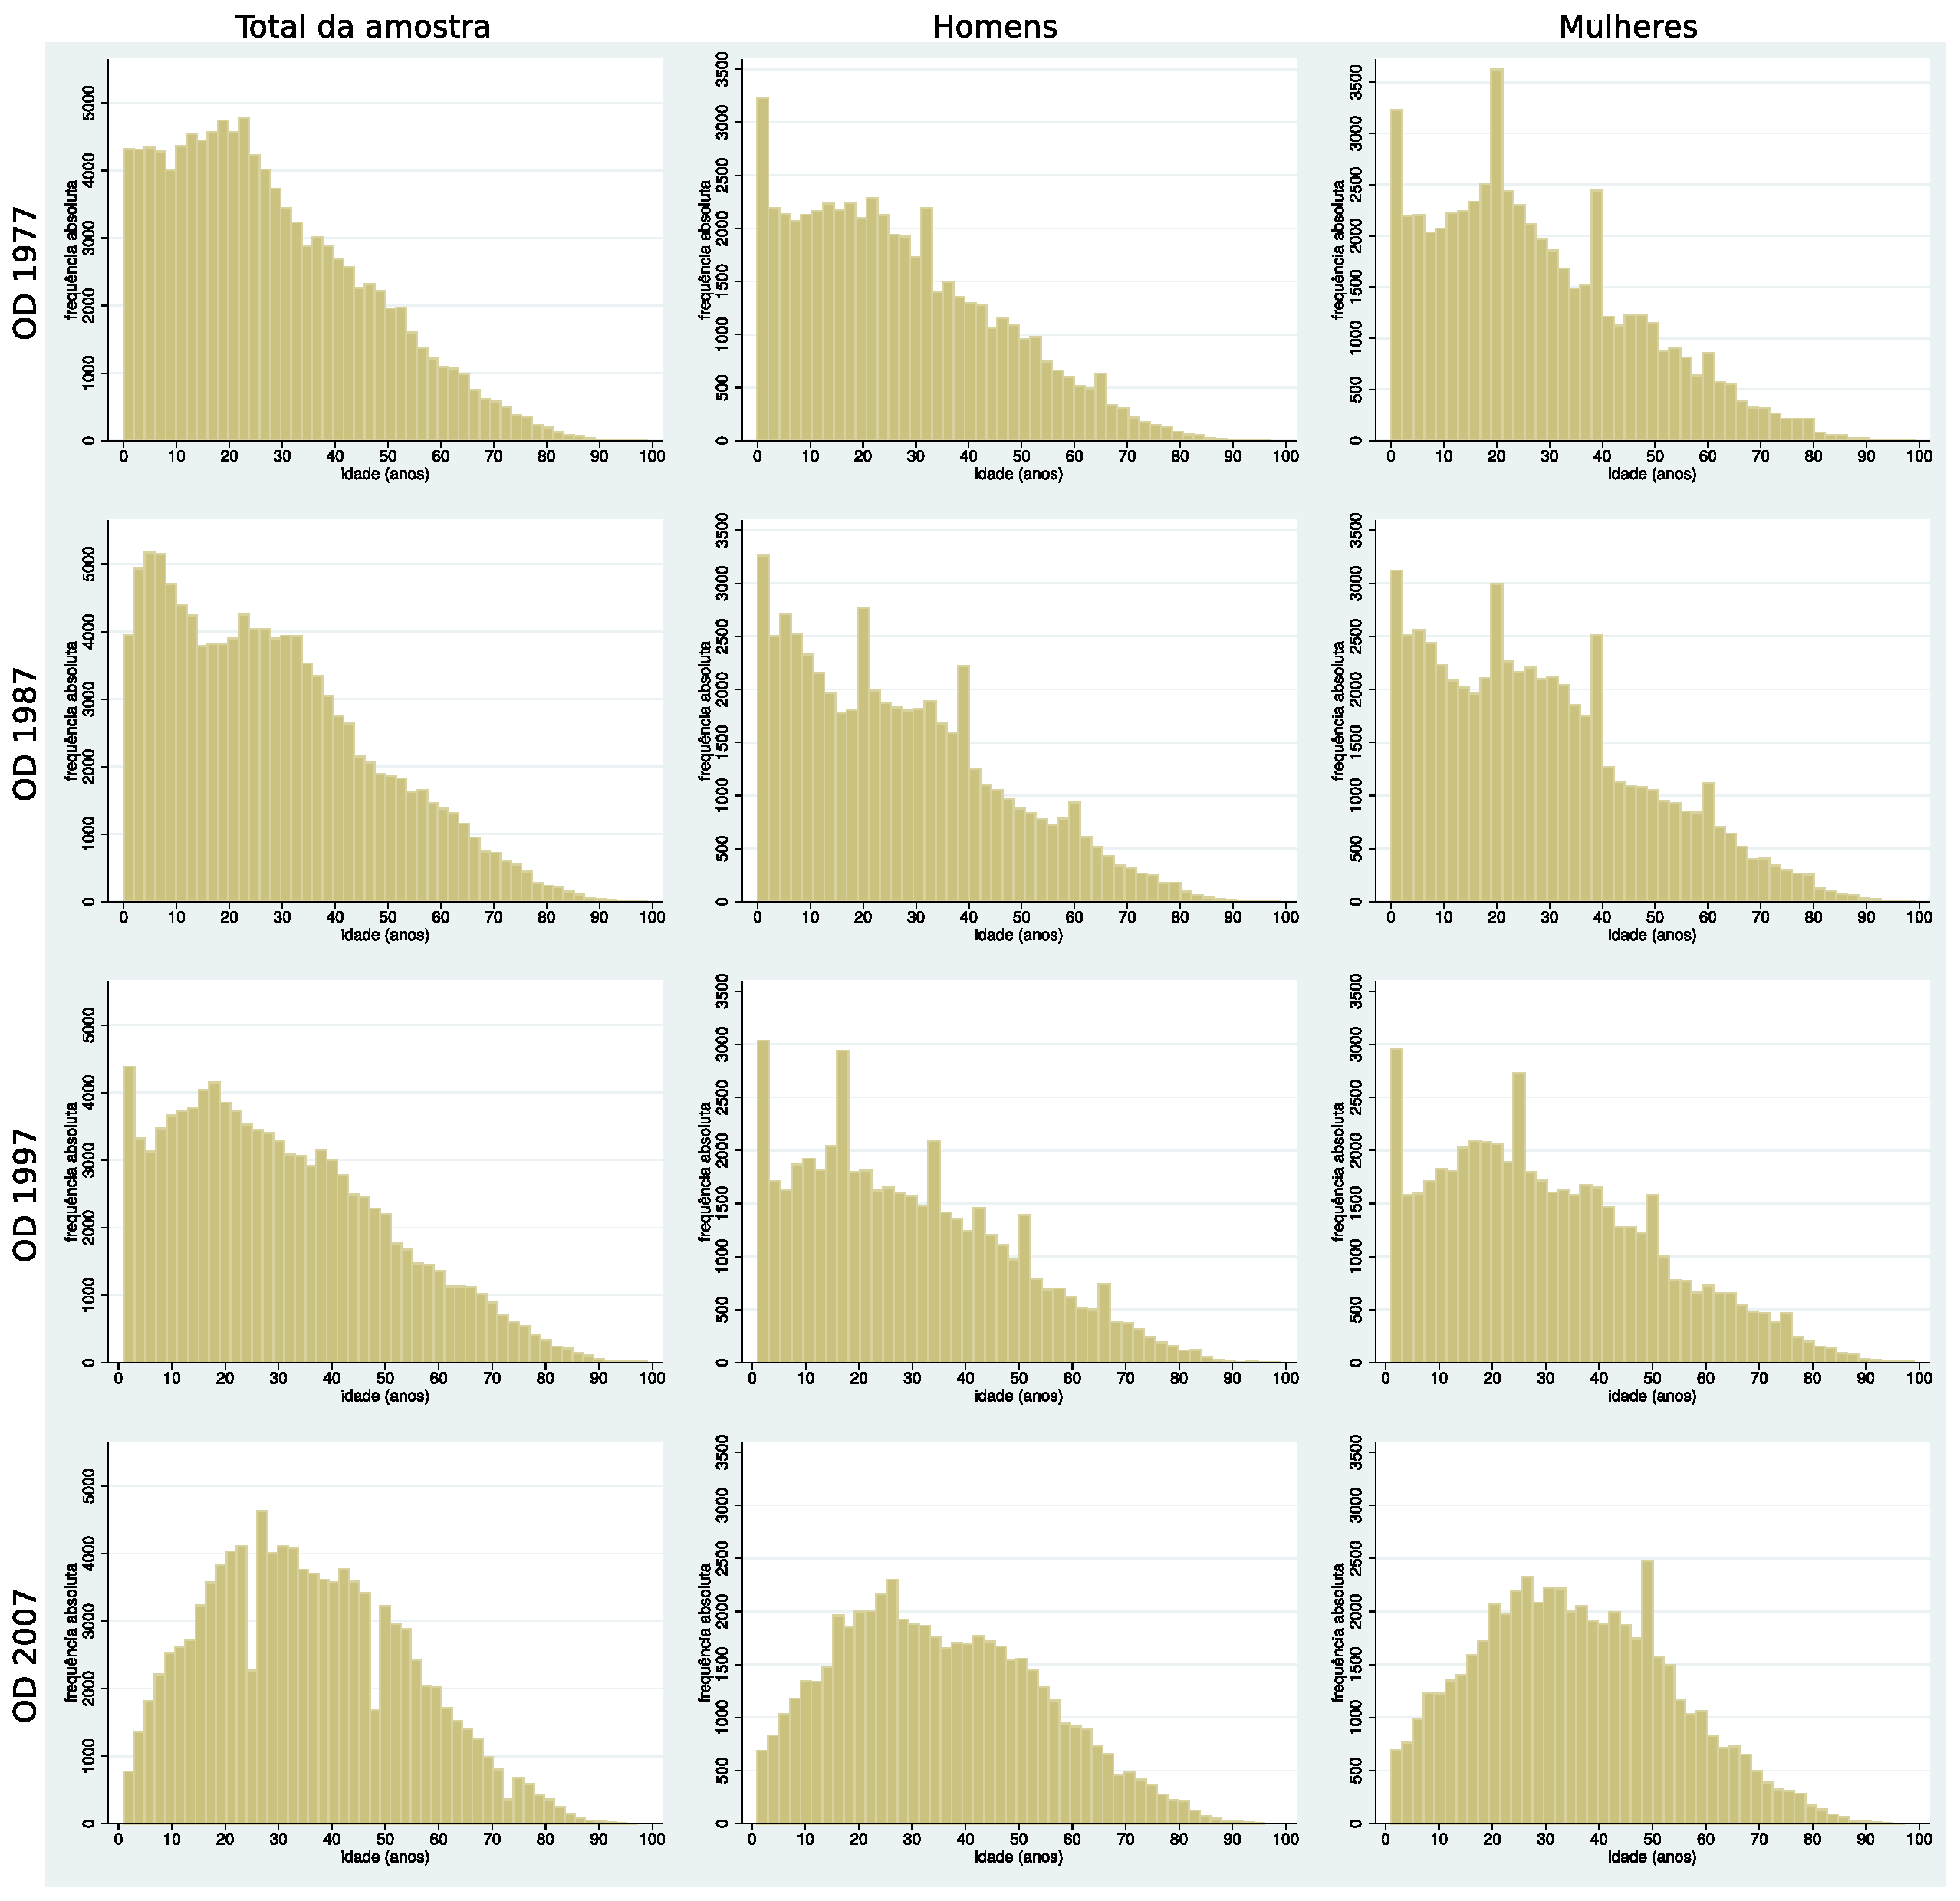
\includegraphics[width=1\textwidth]{./imagens/idade2.eps}%
    \end{center}%
    \fonte{Compilação própria}
\end{grafico}%

\clearpage
No Gráfico \ref{graf:distr-sit-fam} nota-se que para as mulheres houve uma mudança ao longo dessas três décadas. Em 1977, era mais frequente elas ocuparem a posição de filhas (41,81\%), em seguida de cônjuges (36,27\%). A posição de ``pessoa responsável'' pela família é a quarta categoria mais frequente (6,32\%), de seis. Tal distribuição permanece semelhante em 1987. Em 1997, no entanto, a posição de ``pessoa responsável'' pela família (11,13\%) já quase se equipara à posição de ``outro parente/agregado(a)'' (11,27\%). Em 2007, já é quase um quarto das mulheres entrevistadas que são responsáveis por suas famílias (24,21\%), representando aumento de quase 4 vezes em relação aos percentuais de 1977. O percentual de mulheres cônjuges/companheiras pouco se altera ao longo do tempo, permanecendo na faixa dos 35\%. Há diminuição da posição de empregado(a) doméstico(a) para ambos sexos, mas a queda é mais acentuada para mulheres (da ordem de 8 vezes entre 1977 e 2007) do que para homens (queda em 2007 para cerca da metade do valor de 1977). Existe, também, queda da frequência daqueles que se declaram na posição de filho(a) ou enteado(a) tanto para homens como para mulheres - em ordem de grandeza próxima: cerca de 8\% para mulheres e 10\% para homens. Isso pode ser reflexo da diminuição das taxas de fecundidade%
\footnote{Por ``taxa de fecundidade total'' entende-se o número médio de filhos que teria uma mulher de uma coorte hipotética (15 e 49 anos de idade) ao final de seu período reprodutivo. Fonte: IBGE. Disponível em: \url{http://www.ibge.gov.br/home/estatistica/populacao/condicaodevida/indicadoresminimos/conceitos.shtm\#tf}} da população (ver Tabela \ref{tab:taxa-fecund}). Entre os homens percebe-se que houve crescimento entre aqueles com posição de ``pessoas responsável'' de cerca de 8\%, e também dos que declaram-se cônjuge/companheiro (cerca de 20 vezes) - esta última constatação é coerente com o fato de mais mulheres serem a principal fonte de renda doméstica, ou seja, a ``pessoa responsável'' da família.

\begin{table}[htb]
    \IBGEtab{%\renewcommand{\arraystretch}{1.5}%%\ABNTEXfontereduzida%
	    \renewcommand{\arraystretch}{1.5}
        \caption{Evolução das taxas de fecundidade no Brasil, de 1970 a 2010}
		\label{tab:taxa-fecund}
    }{%
	    \begin{tabular}{P{5.00cm} P{1.50cm} P{1.50cm} P{1.50cm} P{1.50cm} P{1.50cm}}
            \toprule
	           \headerTabCenterCell{Ano} &
   	           \headerTabCenterCell{1970} &
   	           \headerTabCenterCell{1980} &
   	           \headerTabCenterCell{1991} &
   	           \headerTabCenterCell{2000} &
   	           \headerTabCenterCell{2010} \\
		    \midrule \midrule
				Taxa de fecundidade (Brasil)&
				5,8&
				4,4&
				2,7&
				2,4&
		        1,9\\
			\midrule
				Taxa de fecundidade (Sudeste)&
				4,6&
				3,2&
				2,4&
				2,1&
		        1,7\\
			\midrule
				Taxa de fecundidade (São Paulo)&
				3,94&
				3,24&
				2,28&
				2,05&
		        1,67\\
			\bottomrule	
		\end{tabular}
    }{%
		\fonte{Compilação a partir de dados dos censos do IBGE disponíveis em \url{http://seculoxx.ibge.gov.br/populacionais-sociais-politicas-e-culturais/busca-por-palavra-chave/populacao/810-fecundidade} Acesso em 17 de novembro de 2014}
		\nota{Ao analisar as taxas de fecundidades para as Grandes Regiões, nota-se que o Sudeste tem os menores percentuais de mulheres que tiveram filhos em todos os subgrupos etários.}
		}
\end{table}

É possível que essa transformação dos papeis sociais desempenhados por homens e mulheres dentro do núcleo familiar ao longo das últimas décadas altere de maneira significativa os padrões de mobilidade de ambos grupos.

\clearpage

\begin{grafico}[htb]%
    \caption{\label{graf:distr-sit-fam}Distribuição da situação familiar de respondentes das Pesquisas OD 1977, 1987, 1997 e 2007, por sexo}%
    \begin{center}%
        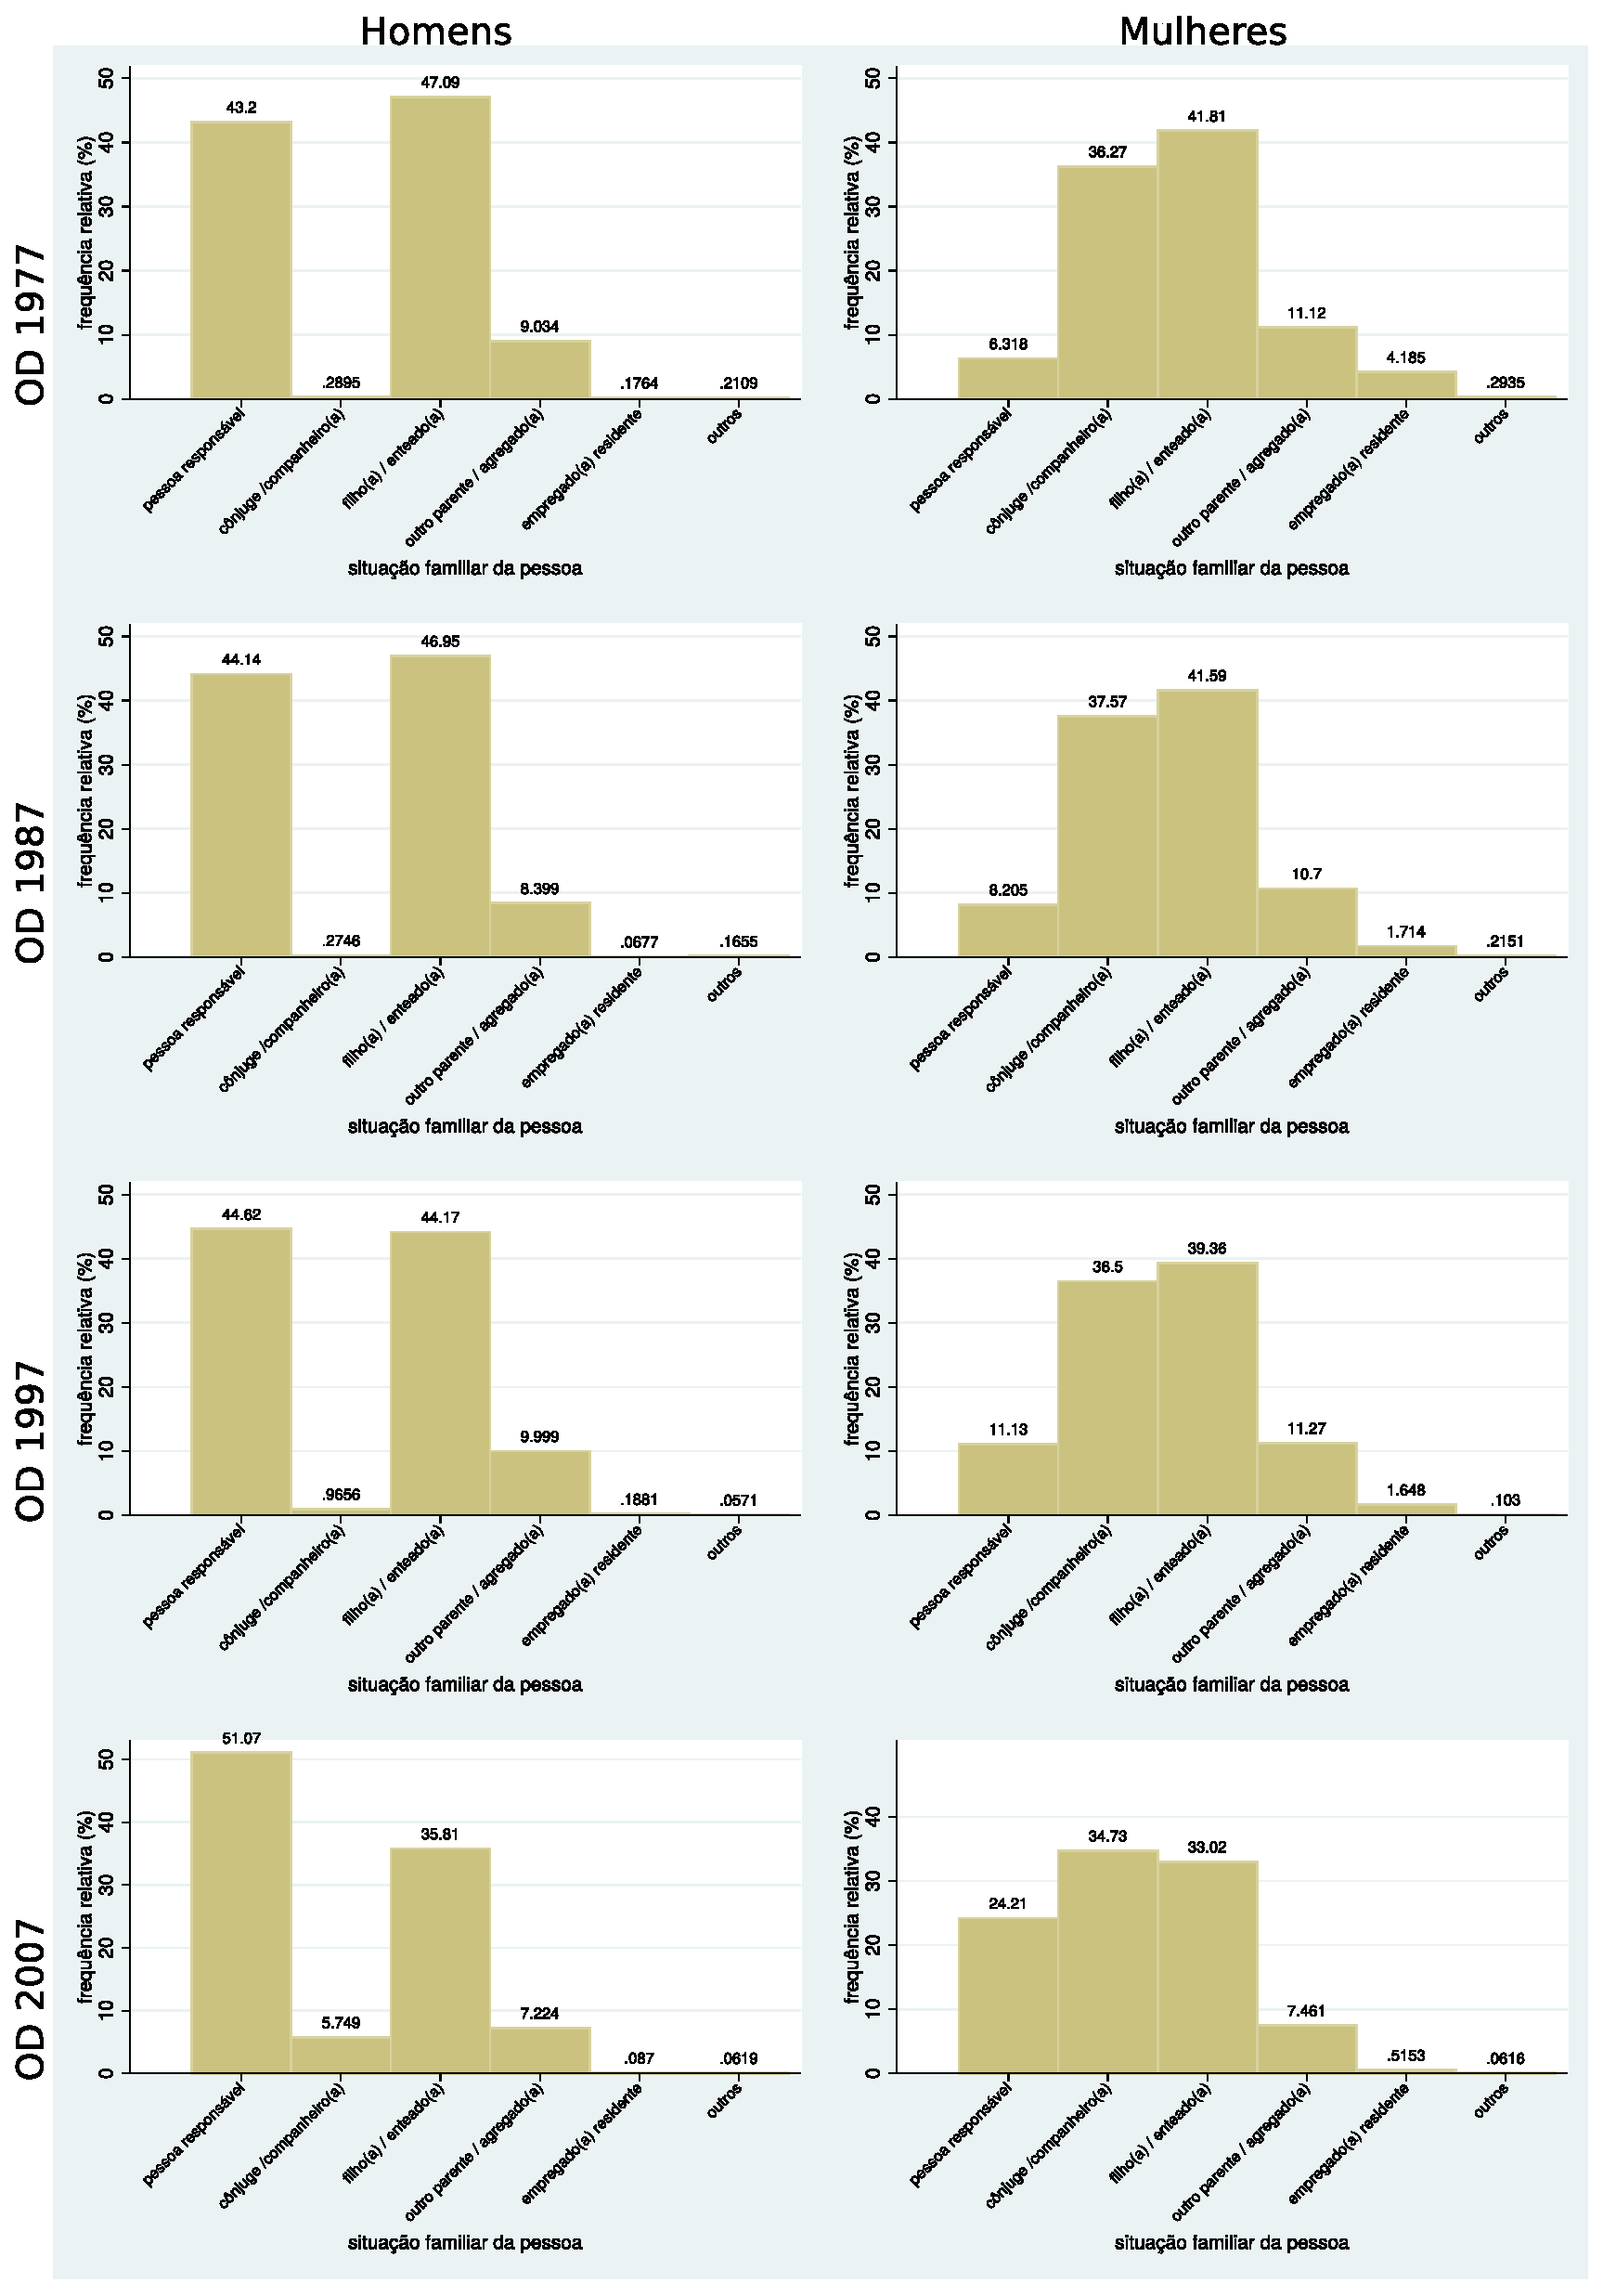
\includegraphics[width=1\textwidth]{./imagens/sitfam2.eps}%
    \end{center}%
    \fonte{Compilação própria}
\end{grafico}%

\clearpage

No Gráfico \ref{graf:distr-grau-instr} nota-se que em 1977 tanto homens como mulheres dispunham de pouco tempo de escolaridade - cerca de três quartos da população ou era analfabeta ou possuía no máximo o fundamental incompleto. Nessa época, nos três níveis de instrução superiores a esse os homens tinham índices maiores que as mulheres. O grau de instrução da população vai aumentando e em 1987, o grau de escolarização feminino é levemente superior ao masculino nas categorias ``fundamental completo / médio incompleto'' e ``médio completo / superior incompleto''. Na categoria ``superior completo'' o grau de instrução masculino é um pouco superior, situação que se inverte em 2007. Neste último ano de análise, as mulheres apresentam maiores percentuais nos dois níveis de maior grau de instrução e os homens, nos dois níveis de menor grau de instrução. Mesmo assim, as marcas para ambos são bastante semelhantes e indicam esforços de políticas públicas no sentido de universalizar os Ensinos Fundamental e Médio no Brasil \ref{tab:grau-instr-ef-em}.

\begin{table}[htb]
    \IBGEtab{%\renewcommand{\arraystretch}{1.5}%%\ABNTEXfontereduzida%
	    \renewcommand{\arraystretch}{1.5}
        \caption{Crescimento de matrículas no Ensino Fundamental e Ensino Médio, no Brasil, entre 1975 e 2005}
		\label{tab:grau-instr-ef-em}
    }{%
	    \begin{tabular}{P{2.00cm} P{4.00cm} P{4.00cm}}
            \toprule
	           \headerTabCenterCell{Ano} &
   	           \headerTabCenterCell{Matrículas no Ensino Fundamental} &
   	           \headerTabCenterCell{Matrículas no Ensino Médio}\\
		    \midrule \midrule
				1975&
		    	100*&
				100*\\
			\midrule
				1980&
				115,6&
		        113,1\\
			\midrule
				1990&
				141,0**&
		        180,8\\
			\midrule
				1996&
				169,5&
		        296,4\\
			\midrule
				2000&
				182,7&
		        423,2\\
			\midrule
				2005&
				171,5&
		        466,5\\
			\bottomrule	
		\end{tabular}
    }{%
		\fonte{Adaptado de \citeauthoronline{OLIVEIRA2007} (\citeyear{OLIVEIRA2007})}
		\nota{* Tomou-se por referência o ano de 1975 (1975=100). 
		** O valor refere-se ao ano de 1989.}
	}
\end{table}

O grau de instrução ter se elevado entre 1977 e 2007 influencia não apenas a empregabilidade e, eventualmente, as viagens motivo trabalho. O principal impacto esperado desse fenômeno dá-se nas viagens motivo escola - realizadas por um contingente de pessoas cada vez maior, mais diverso e contendo mais faixas etárias.

\begin{grafico}[htb]%
    \caption{\label{graf:distr-grau-instr} Distribuição do grau de instrução de respondentes das Pesquisas OD 1977, 1987, 1997 e 2007, por sexo}%
    \begin{center}%
        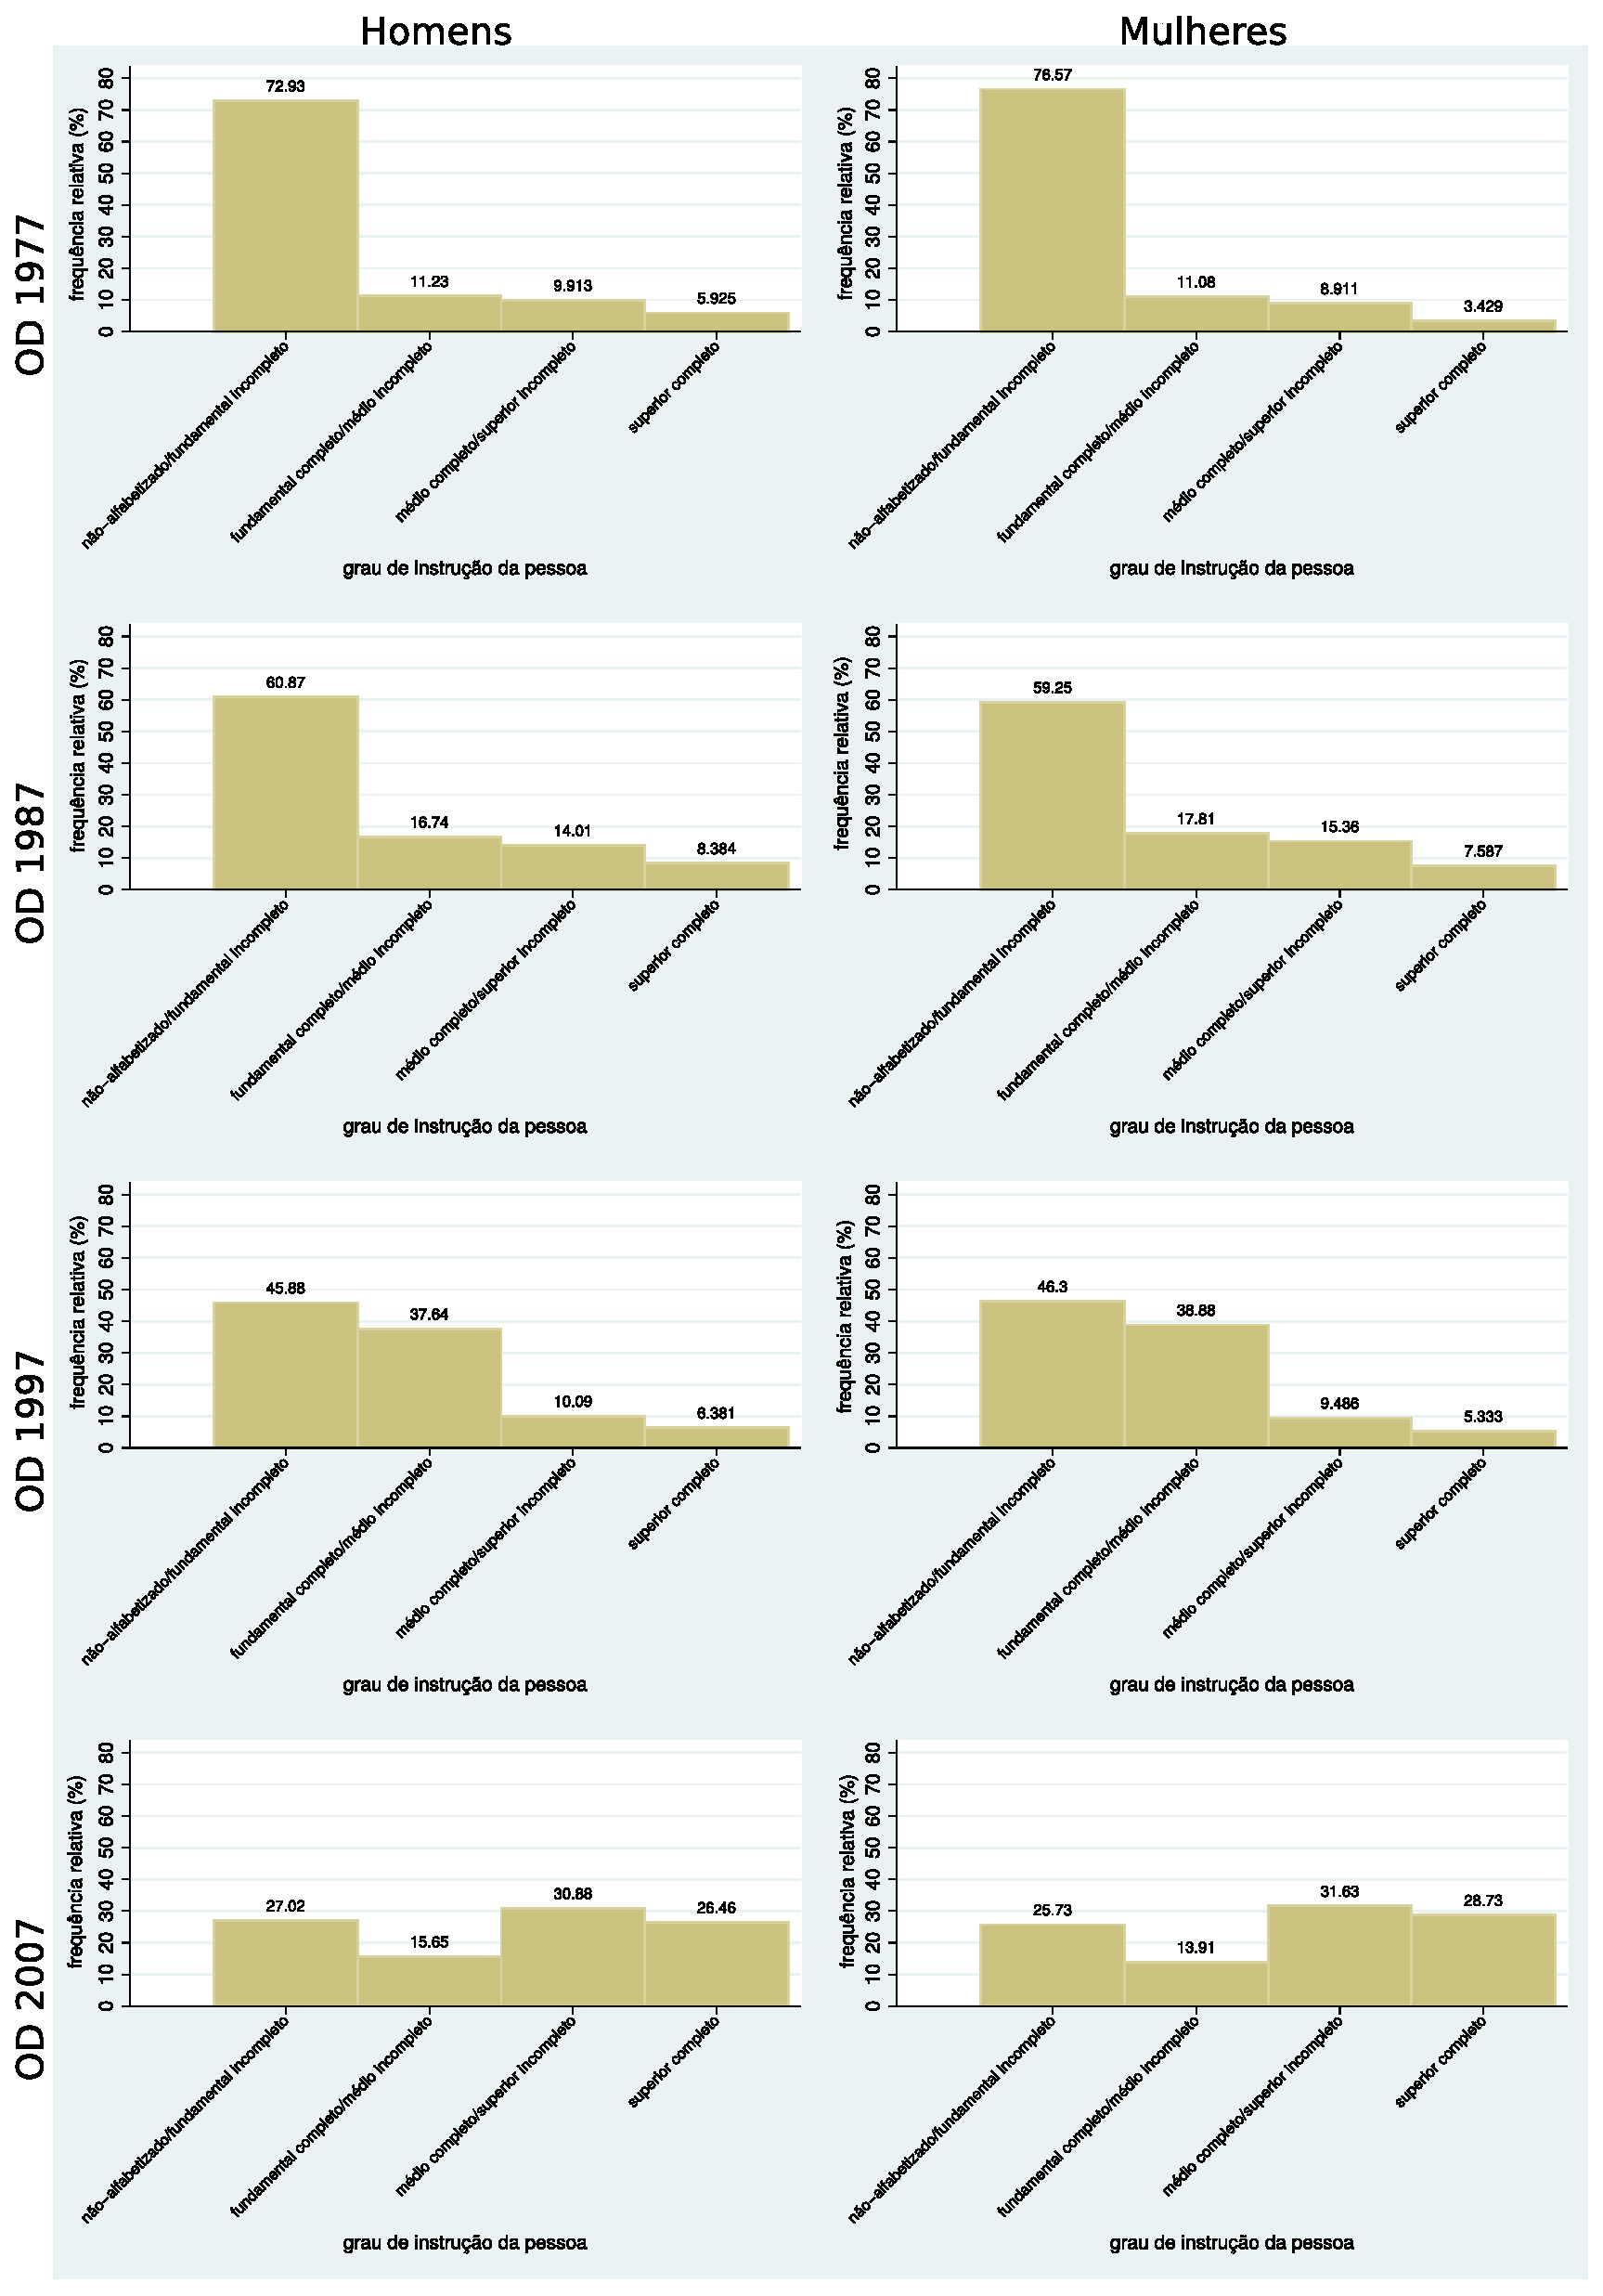
\includegraphics[width=1\textwidth]{./imagens/grauinstr2.eps}%
    \end{center}%
    \fonte{Compilação própria}
\end{grafico}%

\clearpage
O grupo de análises que se segue busca compreender como essa amostra se comporta em termo de viagens realizadas, em cada ano e diferencialmente entre os anos, olhando para tanto variáveis como duração das viagens e número de viagens realizadas.

%Dentro deste segundo grupo de análises foi de interese buscar verificiar se a variável explicativa sexo era relevante para explicar tanto a duração como o número de viagens. Para tanto foram feitas regressões lineares simples e seus resultados são apresentados na Seção \ref{sec:analises-preliminares}. Também há interesse em verificar se existe alguma diferença estatisticamente significativa nos padrões de deslocamento entre os sexos, para cada \emph{cross-section}. Isso foi feito feito tomando como hipótese nula que as médias de ambos sexos eram iguais, para as variáveis dependentes analisadas. Essa hipótese foi testada e os resultados também são apresentados na Seção \ref{sec:analises-preliminares}.

O Gráfico \ref{graf:distr-dur-viag} foi construído considerando-se apenas as viagens cuja duração fosse igual ou superior a 5 minutos. Em todos os anos, para homens e para mulheres, percebem-se alguns picos que ocorrem nos valores múltiplos de cinco minutos. Isso porque a duração de viagem é aquela percebida e declarada pelo(a) respondente. Em 1977, a duração das viagens mais curtas (como 5 e 30 minutos) era menos frequente entre as mulheres (13\% e 14\%, respectivamente) do que entre os homens (26\% e 15\%). Em 1987 as viagens de 5 minutos passam a ser mais frequentes entre mulheres (32\%) do que entre homens (26,5\%). Essa situação se inverte em 1997 e retorna em 2007.
Em todos os anos as viagens mais longas (de 60 e 90 minutos) são mais frequentes entre os homens do que entre as mulheres.
Na Tabela \ref{tab:dur-med-viag} são apresentadas as durações médias de viagens para homens e mulheres. As médias de homens são superiores às das mulheres, ao nível de significância estatística de 5\%. É possível perceber que a duração média de viagem para ambos vem crescendo e a diferença entre esses grupos vem diminuindo.

\begin{table}[htb]
    \IBGEtab{%\renewcommand{\arraystretch}{1.5}%%\ABNTEXfontereduzida%
%	    \renewcommand{\arraystretch}{1.5}
        \caption{Duração média de viagem, por sexo, por ano}
		\label{tab:dur-med-viag}
    }{%
	    \begin{tabular}{P{1.00cm} P{2.00cm} P{2.00cm} P{3.00cm} P{3.00cm} P{3.00cm}}
            \toprule
	           \headerCenterCell{Ano} &
   	           \headerCenterCell{Duração Média de Viagem para Mulheres (min)} &
   	           \headerCenterCell{Duração Média de Viagem para Homens (min)} &
   	           \headerCenterCell{Desvio Padrão da Duração Média de Viagem para Mulheres}&   	           
   	           \headerCenterCell{Desvio Padrão da Duração Média de Viagem para Homens} &   	           
   	           \headerCenterCell{Diferença entre as durações médias (Dur\_mulher - Dur\_homem)}\\
		    \midrule \midrule
				1977&
		    	29,23&
		    	33,27&
		    	28,52&
		    	31,69&
				-4,04\\
			\midrule
				1987&
				30,27&
				35,82&
				29,29&
				33,11&
		        -5,55\\
			\midrule
				1997&
				32,09&
				35,61&
				30,83&
				33,90&
		        -3,52\\
			\midrule
				2007&
				35,35&
				37,39&
				32,76&
				33,87&
		        -2,04\\
			\bottomrule	
		\end{tabular}
    }{%
		\fonte{Elaboração própria}
	}
\end{table}

Ao fazer a regressão linear da variável duração (valores superiores a 5 minutos) unicamente em função da variável explicativa sexo, para todos anos, os p-valores relativos ao coeficientes da variável \emph{dummy} explicativa foram inferiores a 0,05, o que dá indícios de que a variável sexo é umas das variáveis de análise importantes para explicar o tempo dispendido nos deslocamentos.

\begin{grafico}[htb]%
    \caption{\label{graf:distr-dur-viag}Distribuição da duração de viagens de respondentes das Pesquisas OD 1977, 1987, 1997 e 2007, por sexo}%
    \begin{center}%
        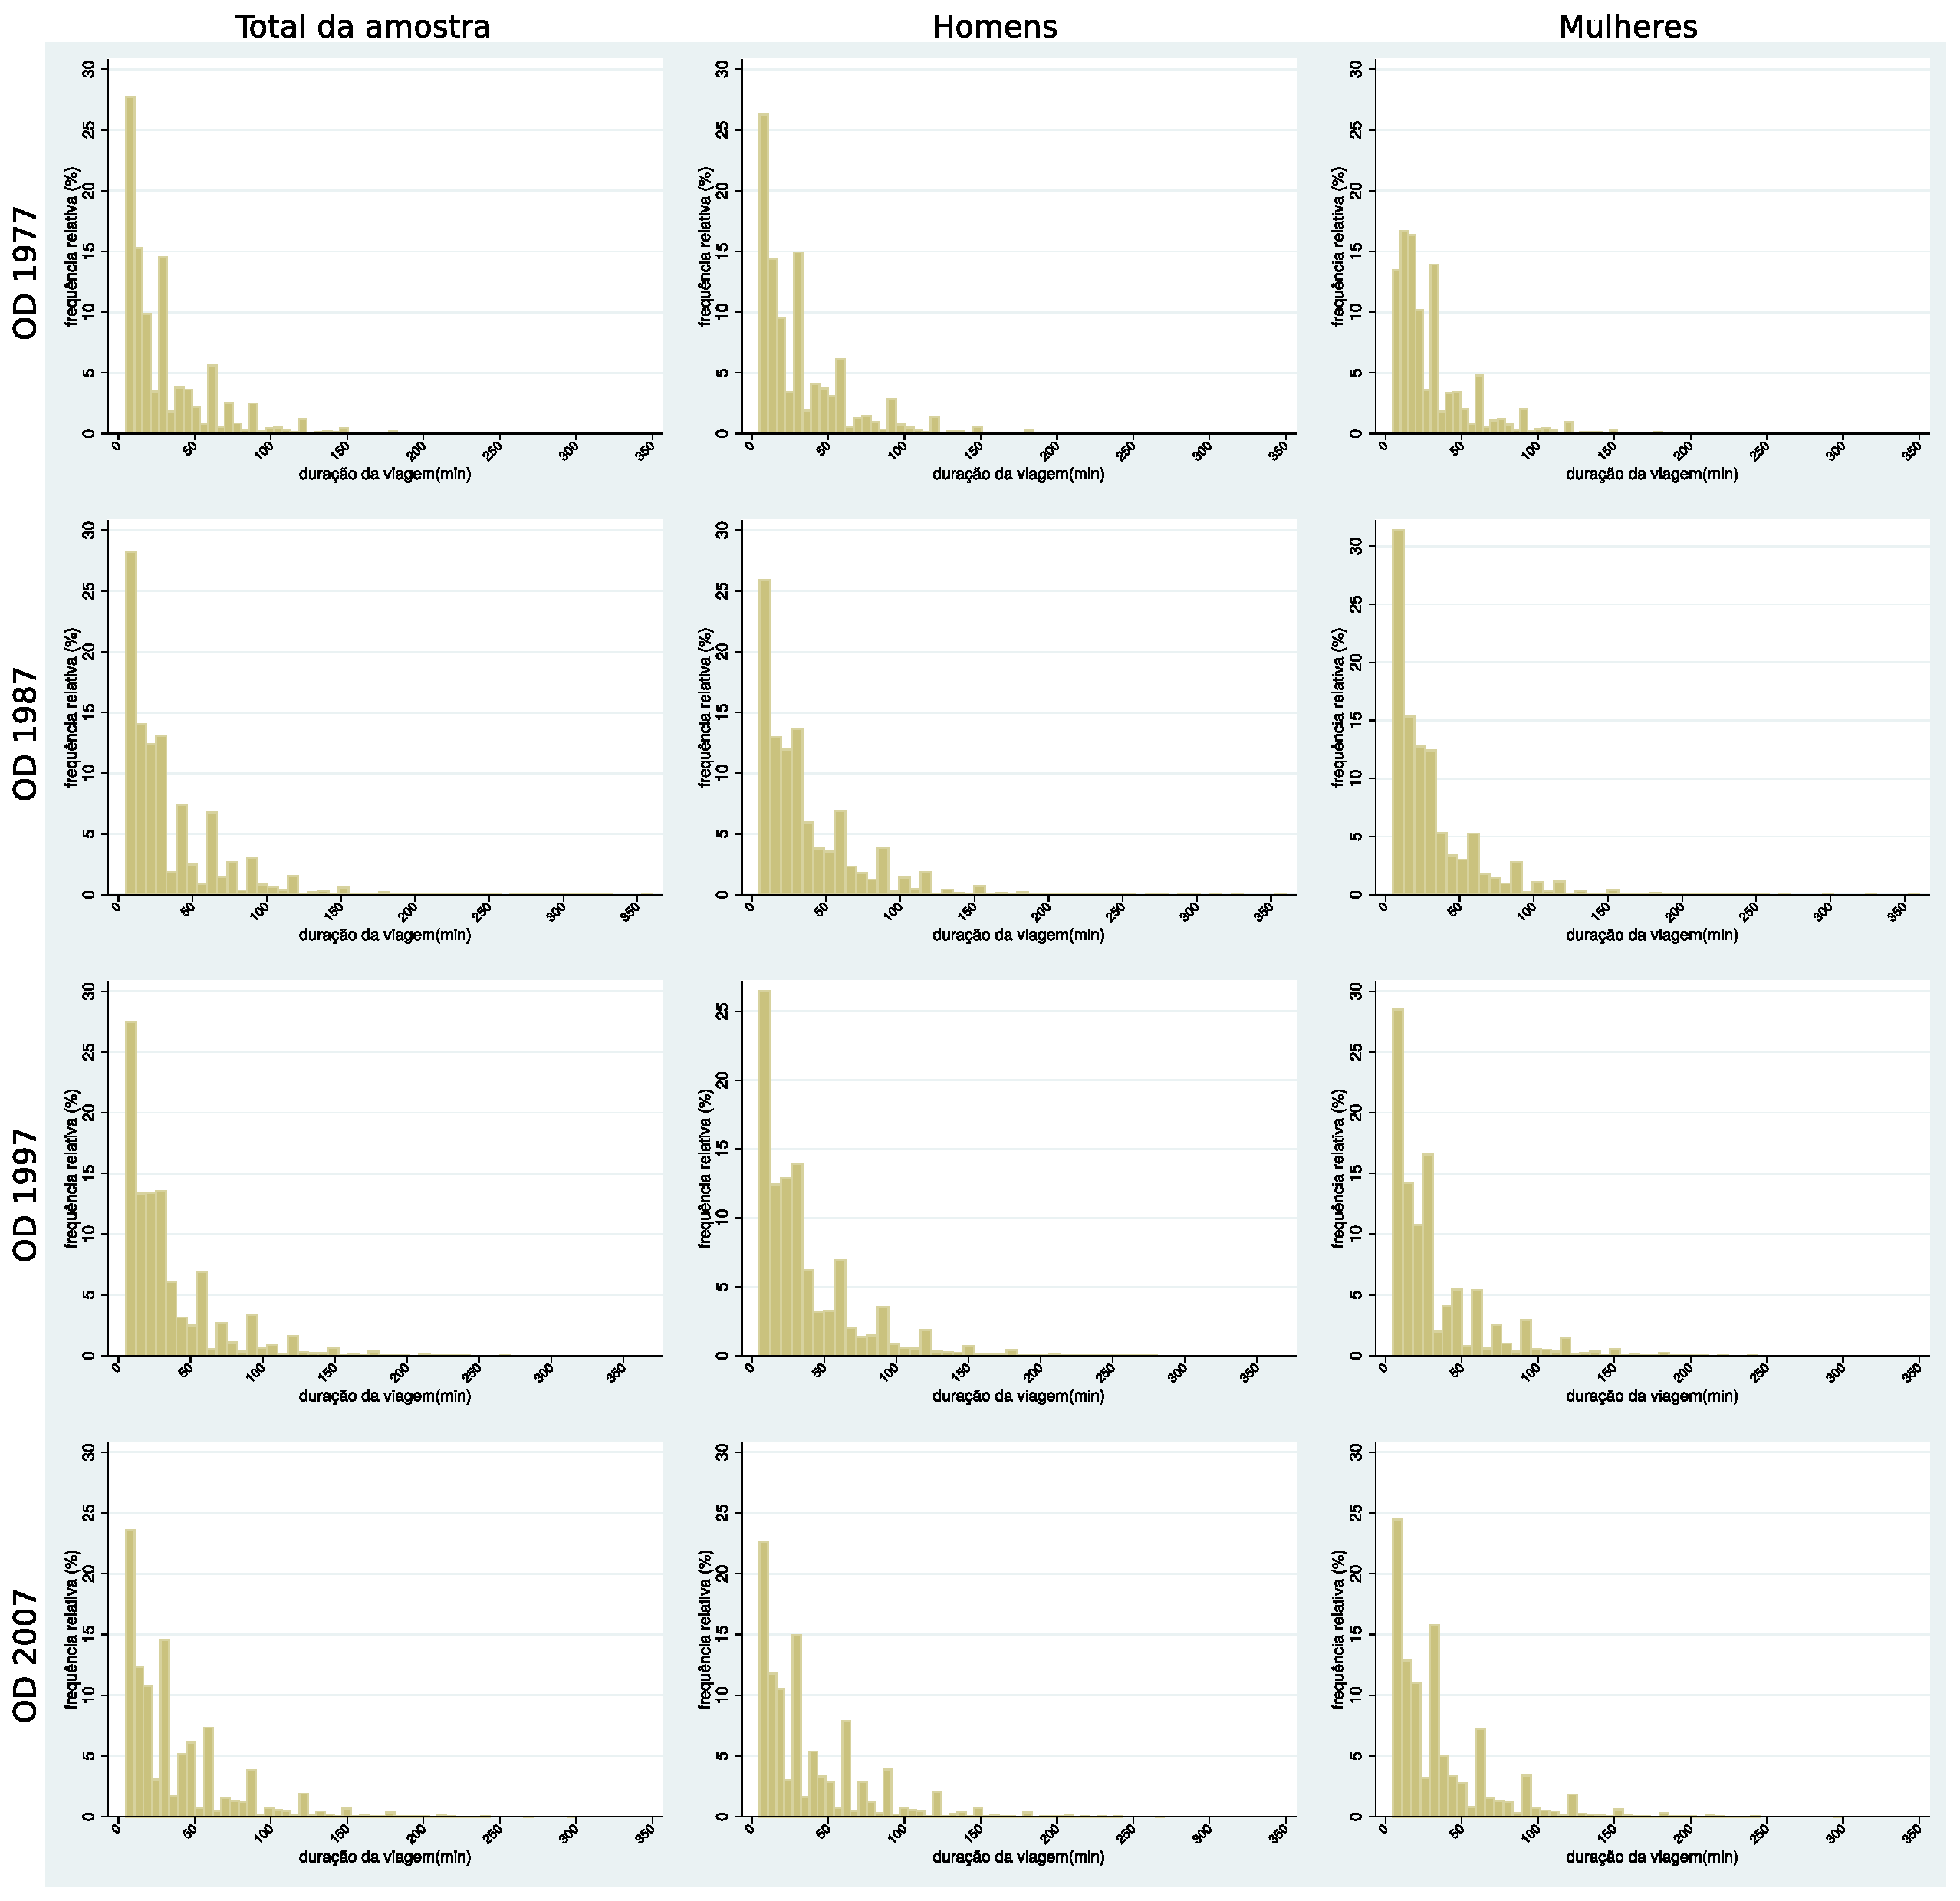
\includegraphics[width=1.1\textwidth]{./imagens/duradeviagens2.eps}%
    \end{center}%
    \fonte{Compilação própria}
\end{grafico}%

\clearpage
Analisando a distribuição do número de viagens por pessoa, conforme já era de se esperar, para quem faz viagem no dia da pesquisa (número de viagem é não nulo) existe a predominância do valor 2, ou seja, são pessoas que saem de suas residências com um propósito único (trabalhar, estudar, fazer compras) e depois retornam à residência após a atividade. O que vale analisar no Gráfico \ref{graf:distr-num-viag} é a relação entre as viagens nulas (não sai de casa) e as viagens de ida e volta (valores iguais a 2). Para homens, o número de viagens nulo é menos frequente que o número de viagens de valor 2 para todos anos de análise. Já para as mulheres, em 1977 as viagens nulas eram a maioria, indicando certa fixitude delas na residência. Essa porcentagem vai diminuindo e a porcentagem no número de viagens igual a 2 vai crescendo, ficam próximas em 1997 e, em 2007, inverte-se a situação observada em 1977. Coincidentemente com a conquista de maior participação no mercado de trabalho, essa alteração pode ser um indício de que as mulheres ganharam mobilidade, restringindo-se menos ao espaço doméstico.

Na Tabela \ref{tab:num-med-viag} são apresentados os números médios de viagens para homens e mulheres. As médias de homens são superiores às das mulheres, ao nível de significância estatística de 5\%. O número médio de viagens para os homens caiu entre 1977 e 1997, voltando a subir em 2007. Isso pode ter se dado em função de uma diminuição no nível de postos de trabalho ocupados por homens no período. O número médio de viagens para as mulheres aumentou desde 1977 até 2007. Apesar dessa mudança de tendência no padrão masculino, a diferença entre os gêneros só tem diminuído.

Ao fazer a regressão linear da variável total de viagens da pessoa unicamente em função da variável explicativo sexo, para todos anos os p-valores foram inferiores a 0,05, o que mostra indícios de que a variável sexo é umas das variáveis de análise para explicar a quantidade de viagens feitas pelo indivíduo.

%\hl{verificar se é preciso apresentar os resultados de teste F e teste t p/ comparação de médias OU ANOVA com prévia averiguaçaõ de matrizes de covariância + teste Levene + teste normalidade (não vai passar...)}

\begin{table}[htb]
    \IBGEtab{%\renewcommand{\arraystretch}{1.5}%%\ABNTEXfontereduzida%
%	    \renewcommand{\arraystretch}{1.5}
        \caption{Número médio de viagens, por sexo, por ano}
		\label{tab:num-med-viag}
    }{%
	    \begin{tabular}{P{1.00cm} P{2.00cm} P{2.00cm} P{3.00cm} P{3.00cm} P{3.00cm}}
            \toprule
	           \headerCenterCell{Ano} &
   	           \headerCenterCell{Número Médio de Viagem para Mulheres (min)} &
   	           \headerCenterCell{Número Médio de Viagem para Homens (min)} &
   	           \headerCenterCell{Desvio Padrão da Número Médio de Viagem para Mulheres} &   	           
   	           \headerCenterCell{Desvio Padrão do Número Médio de Viagem para Homens} &   	           
   	           \headerCenterCell{Diferença entre os números médios de viagens (Nº\_mulher - Nº\_homem)}\\
		    \midrule \midrule
				1977&
		    	1,40&
		    	2,09&
		    	1,64&
		    	1,92&
				-0,69\\
			\midrule
				1987&
				1,42&
				1,89&
				1,59&
				1,61&
		        -0,47\\
			\midrule
				1997&
				1,53&
				1,79&
				1,63&
				1,60&
		        -0,26\\
			\midrule
				2007&
				1,75&
				1,98&
				1,64&
				1,58&
		        -0,23\\
			\bottomrule	
		\end{tabular}
    }{%
		\fonte{Elaboração própria}
	}
\end{table}


\begin{grafico}[htb]%
    \caption{\label{graf:distr-num-viag}Distribuição do número de viagens por respondente das Pesquisas OD 1977, 1987, 1997 e 2007, por sexo}%
    \begin{center}%
        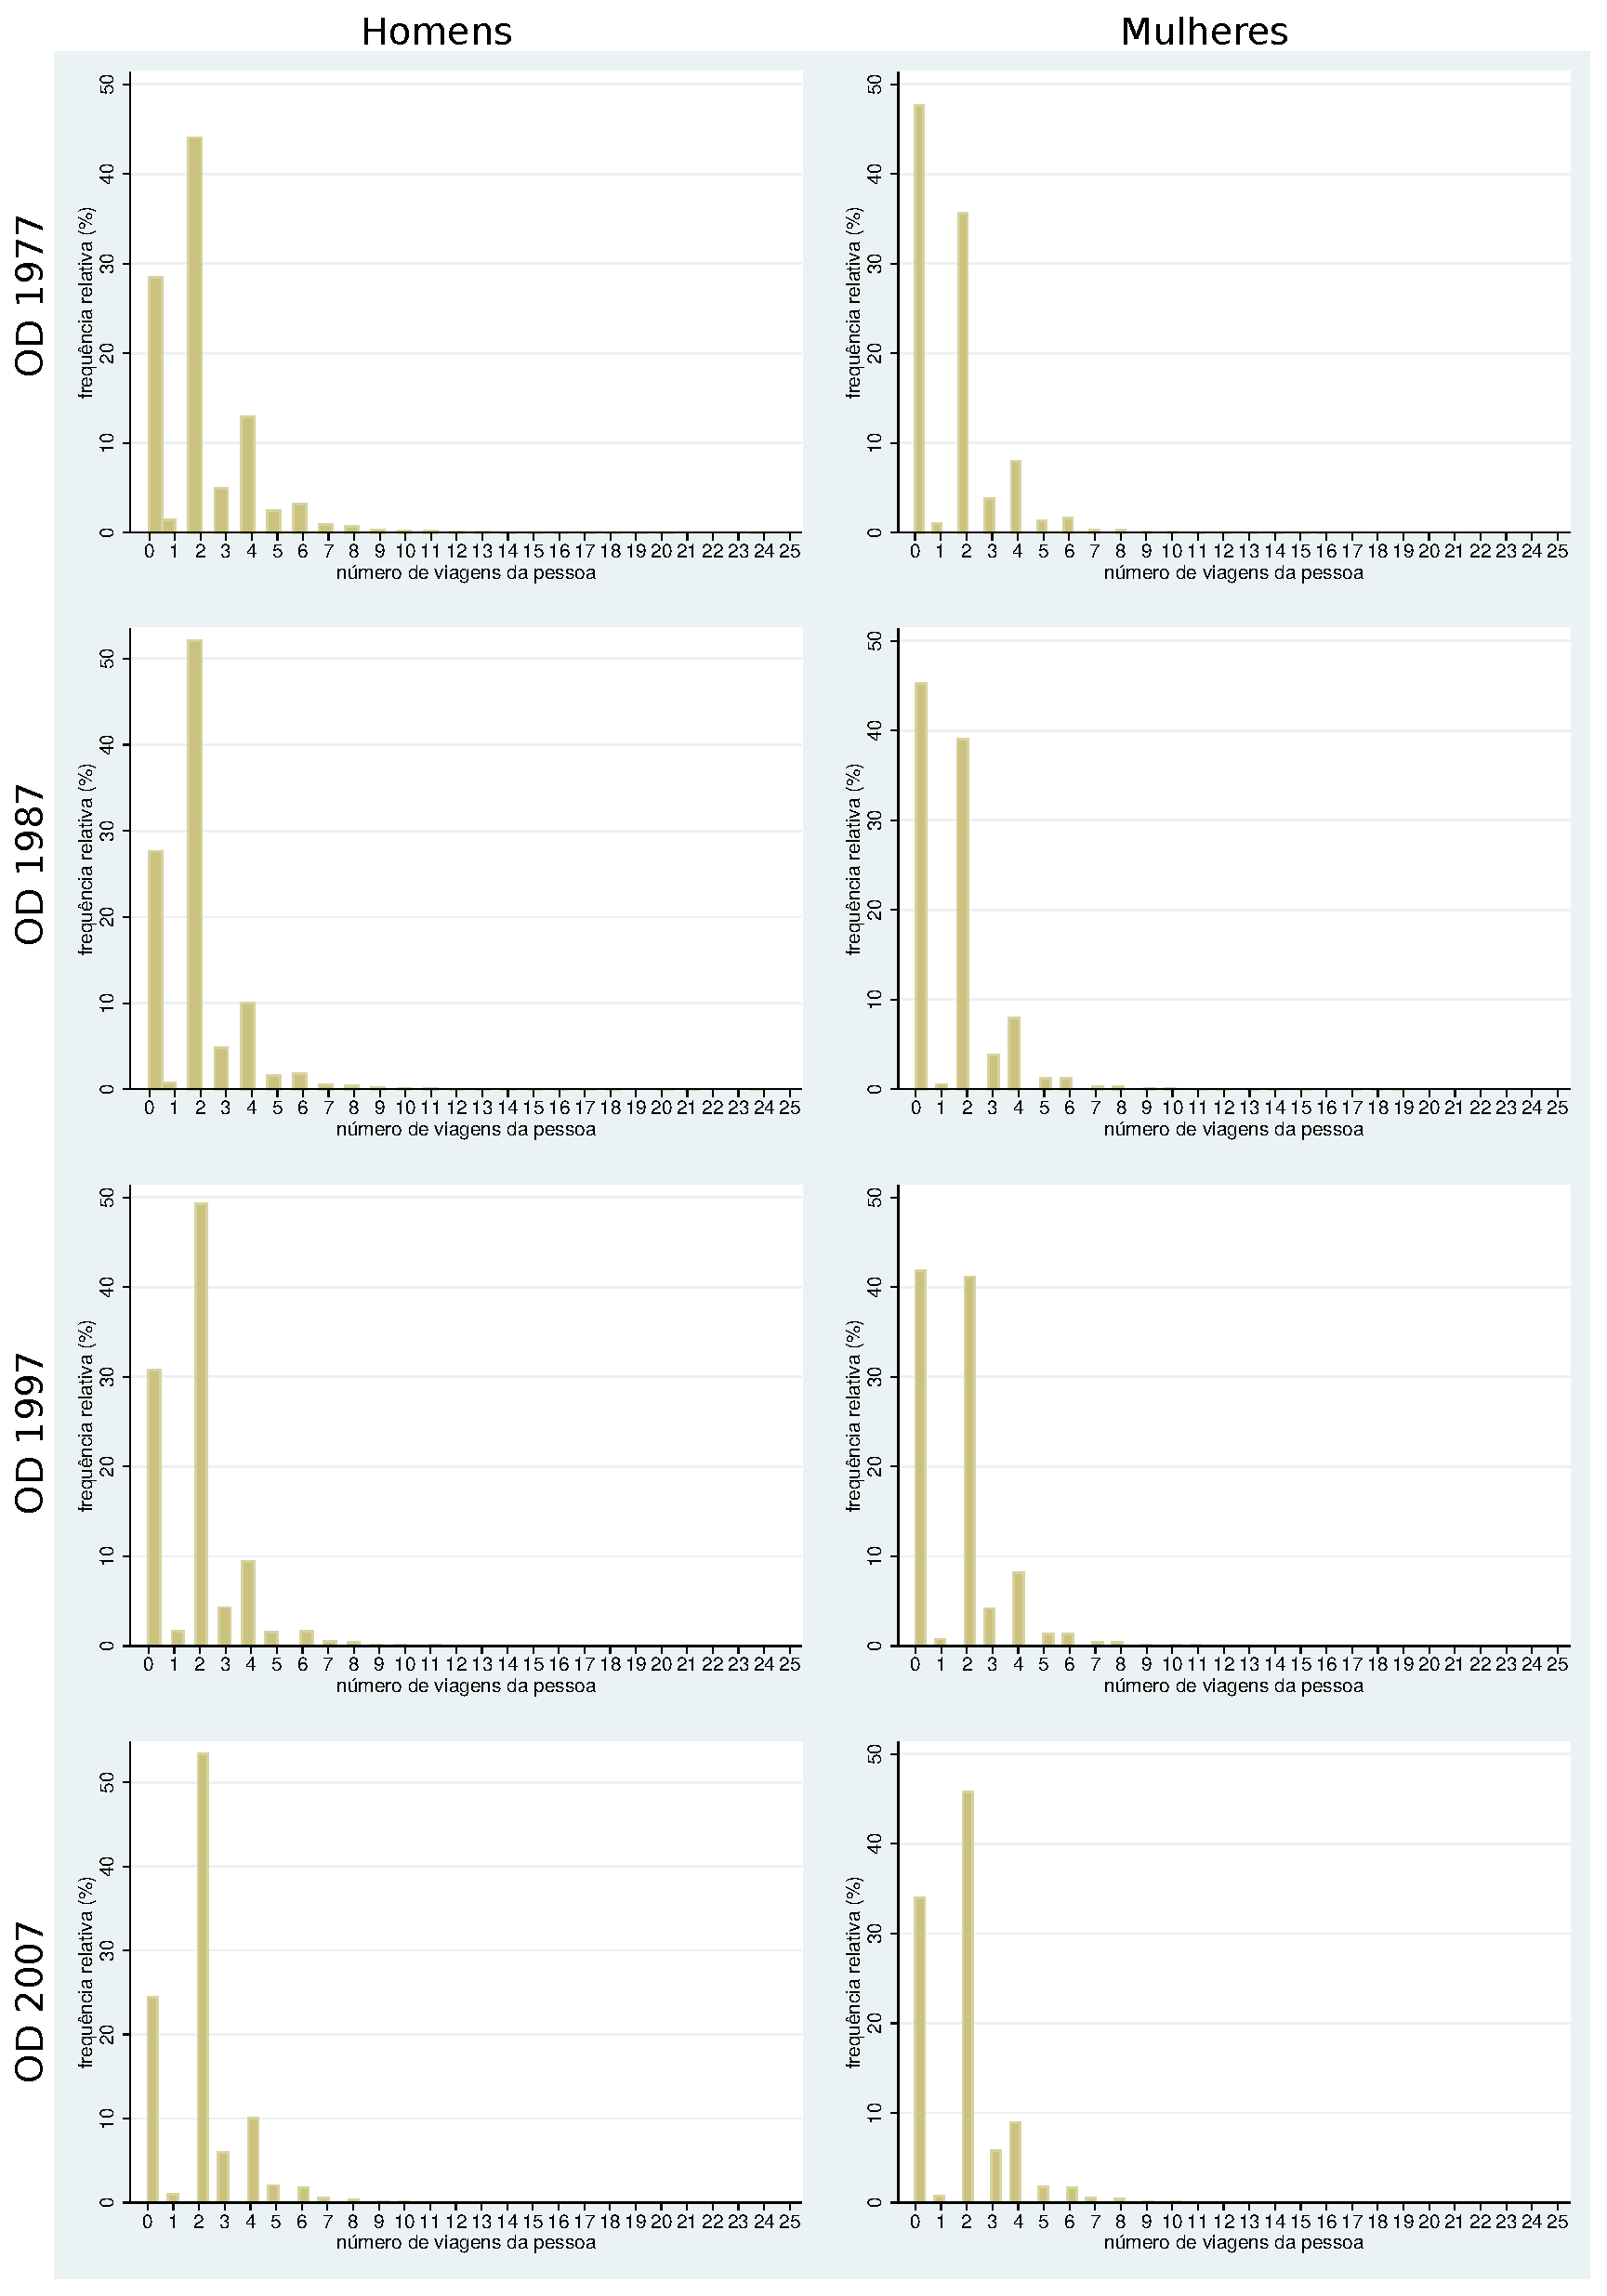
\includegraphics[width=1\textwidth]{./imagens/qtdeviagens2.eps}%
    \end{center}%
    \fonte{Compilação própria}
\end{grafico}%

\clearpage

Tendo em vista as questões apontadas na revisão de literatura a respeito da mobilidade/imobilidade das pessoas e formas de mensurá-la, pretende-se avaliar a distância média das viagens em função das variáveis sexo, idade, renda familiar, renda individual, estado civil e presença de filhos da família \cite{ROSENBLOOM2006,SHEARMUR2006,HANSON2010}. Essa análise ainda não foi possível porque apenas a OD-2007 dispõe das coordenadas de origem e destino das viagens. As demais Pesquisas OD apontam apena a zona de origem e destino das viagens. A distância dessas viagens pode ser calculada a partir dos centroides das zonas, mas optou-se tentar diminuir o grau de imprecisão que essa simplificação implica, adotando os centroides das subzonas, unidades espaciais menores. Porém, as coordenadas dos centroides tanto de zonas como de subzonas não estão disponíveis nos bancos de dados recebidos do Metrô-SP e já se está contatando novamente a empresa para aquisição dessas coordenadas.

